\PassOptionsToPackage{unicode=true}{hyperref} % options for packages loaded elsewhere
\PassOptionsToPackage{hyphens}{url}
\PassOptionsToPackage{dvipsnames,svgnames*,x11names*}{xcolor}
%
\documentclass[10pt,ignorenonframetext,]{beamer}
\usepackage{pgfpages}
\setbeamertemplate{caption}[numbered]
\setbeamertemplate{caption label separator}{: }
\setbeamercolor{caption name}{fg=normal text.fg}
\beamertemplatenavigationsymbolsempty
% Prevent slide breaks in the middle of a paragraph:
\widowpenalties 1 10000
\raggedbottom
\setbeamertemplate{part page}{
\centering
\begin{beamercolorbox}[sep=16pt,center]{part title}
  \usebeamerfont{part title}\insertpart\par
\end{beamercolorbox}
}
\setbeamertemplate{section page}{
\centering
\begin{beamercolorbox}[sep=12pt,center]{part title}
  \usebeamerfont{section title}\insertsection\par
\end{beamercolorbox}
}
\setbeamertemplate{subsection page}{
\centering
\begin{beamercolorbox}[sep=8pt,center]{part title}
  \usebeamerfont{subsection title}\insertsubsection\par
\end{beamercolorbox}
}
\AtBeginPart{
  \frame{\partpage}
}
\AtBeginSection{
  \ifbibliography
  \else
    \frame{\sectionpage}
  \fi
}
\AtBeginSubsection{
  \frame{\subsectionpage}
}
\usepackage{lmodern}
\usepackage{amssymb,amsmath}
\usepackage{ifxetex,ifluatex}
\usepackage{fixltx2e} % provides \textsubscript
\ifnum 0\ifxetex 1\fi\ifluatex 1\fi=0 % if pdftex
  \usepackage[T1]{fontenc}
  \usepackage[utf8]{inputenc}
  \usepackage{textcomp} % provides euro and other symbols
\else % if luatex or xelatex
  \usepackage{unicode-math}
  \defaultfontfeatures{Ligatures=TeX,Scale=MatchLowercase}
\fi
\usetheme[]{Singapore}
\usefonttheme{serif}
% use upquote if available, for straight quotes in verbatim environments
\IfFileExists{upquote.sty}{\usepackage{upquote}}{}
% use microtype if available
\IfFileExists{microtype.sty}{%
\usepackage[]{microtype}
\UseMicrotypeSet[protrusion]{basicmath} % disable protrusion for tt fonts
}{}
\IfFileExists{parskip.sty}{%
\usepackage{parskip}
}{% else
\setlength{\parindent}{0pt}
\setlength{\parskip}{6pt plus 2pt minus 1pt}
}
\usepackage{xcolor}
\usepackage{hyperref}
\hypersetup{
            pdftitle={Module 4: Classification},
            pdfauthor={Stefanie Muff, Department of Mathematical Sciences, NTNU},
            colorlinks=true,
            linkcolor=Maroon,
            filecolor=Maroon,
            citecolor=Blue,
            urlcolor=blue,
            breaklinks=true}
\urlstyle{same}  % don't use monospace font for urls
\newif\ifbibliography
\usepackage{color}
\usepackage{fancyvrb}
\newcommand{\VerbBar}{|}
\newcommand{\VERB}{\Verb[commandchars=\\\{\}]}
\DefineVerbatimEnvironment{Highlighting}{Verbatim}{commandchars=\\\{\}}
% Add ',fontsize=\small' for more characters per line
\usepackage{framed}
\definecolor{shadecolor}{RGB}{248,248,248}
\newenvironment{Shaded}{\begin{snugshade}}{\end{snugshade}}
\newcommand{\AlertTok}[1]{\textcolor[rgb]{0.94,0.16,0.16}{#1}}
\newcommand{\AnnotationTok}[1]{\textcolor[rgb]{0.56,0.35,0.01}{\textbf{\textit{#1}}}}
\newcommand{\AttributeTok}[1]{\textcolor[rgb]{0.77,0.63,0.00}{#1}}
\newcommand{\BaseNTok}[1]{\textcolor[rgb]{0.00,0.00,0.81}{#1}}
\newcommand{\BuiltInTok}[1]{#1}
\newcommand{\CharTok}[1]{\textcolor[rgb]{0.31,0.60,0.02}{#1}}
\newcommand{\CommentTok}[1]{\textcolor[rgb]{0.56,0.35,0.01}{\textit{#1}}}
\newcommand{\CommentVarTok}[1]{\textcolor[rgb]{0.56,0.35,0.01}{\textbf{\textit{#1}}}}
\newcommand{\ConstantTok}[1]{\textcolor[rgb]{0.00,0.00,0.00}{#1}}
\newcommand{\ControlFlowTok}[1]{\textcolor[rgb]{0.13,0.29,0.53}{\textbf{#1}}}
\newcommand{\DataTypeTok}[1]{\textcolor[rgb]{0.13,0.29,0.53}{#1}}
\newcommand{\DecValTok}[1]{\textcolor[rgb]{0.00,0.00,0.81}{#1}}
\newcommand{\DocumentationTok}[1]{\textcolor[rgb]{0.56,0.35,0.01}{\textbf{\textit{#1}}}}
\newcommand{\ErrorTok}[1]{\textcolor[rgb]{0.64,0.00,0.00}{\textbf{#1}}}
\newcommand{\ExtensionTok}[1]{#1}
\newcommand{\FloatTok}[1]{\textcolor[rgb]{0.00,0.00,0.81}{#1}}
\newcommand{\FunctionTok}[1]{\textcolor[rgb]{0.00,0.00,0.00}{#1}}
\newcommand{\ImportTok}[1]{#1}
\newcommand{\InformationTok}[1]{\textcolor[rgb]{0.56,0.35,0.01}{\textbf{\textit{#1}}}}
\newcommand{\KeywordTok}[1]{\textcolor[rgb]{0.13,0.29,0.53}{\textbf{#1}}}
\newcommand{\NormalTok}[1]{#1}
\newcommand{\OperatorTok}[1]{\textcolor[rgb]{0.81,0.36,0.00}{\textbf{#1}}}
\newcommand{\OtherTok}[1]{\textcolor[rgb]{0.56,0.35,0.01}{#1}}
\newcommand{\PreprocessorTok}[1]{\textcolor[rgb]{0.56,0.35,0.01}{\textit{#1}}}
\newcommand{\RegionMarkerTok}[1]{#1}
\newcommand{\SpecialCharTok}[1]{\textcolor[rgb]{0.00,0.00,0.00}{#1}}
\newcommand{\SpecialStringTok}[1]{\textcolor[rgb]{0.31,0.60,0.02}{#1}}
\newcommand{\StringTok}[1]{\textcolor[rgb]{0.31,0.60,0.02}{#1}}
\newcommand{\VariableTok}[1]{\textcolor[rgb]{0.00,0.00,0.00}{#1}}
\newcommand{\VerbatimStringTok}[1]{\textcolor[rgb]{0.31,0.60,0.02}{#1}}
\newcommand{\WarningTok}[1]{\textcolor[rgb]{0.56,0.35,0.01}{\textbf{\textit{#1}}}}
\usepackage{graphicx,grffile}
\makeatletter
\def\maxwidth{\ifdim\Gin@nat@width>\linewidth\linewidth\else\Gin@nat@width\fi}
\def\maxheight{\ifdim\Gin@nat@height>\textheight\textheight\else\Gin@nat@height\fi}
\makeatother
% Scale images if necessary, so that they will not overflow the page
% margins by default, and it is still possible to overwrite the defaults
% using explicit options in \includegraphics[width, height, ...]{}
\setkeys{Gin}{width=\maxwidth,height=\maxheight,keepaspectratio}
\setlength{\emergencystretch}{3em}  % prevent overfull lines
\providecommand{\tightlist}{%
  \setlength{\itemsep}{0pt}\setlength{\parskip}{0pt}}
\setcounter{secnumdepth}{0}

% set default figure placement to htbp
\makeatletter
\def\fps@figure{htbp}
\makeatother

\usepackage{multirow}

\title{Module 4: Classification}
\providecommand{\subtitle}[1]{}
\subtitle{TMA4268 Statistical Learning V2021}
\author{Stefanie Muff, Department of Mathematical Sciences, NTNU}
\date{February 1st and 2nd, 2021}

\begin{document}
\frame{\titlepage}

\begin{frame}

Last update: February 1st, 2021

\end{frame}

\begin{frame}{Acknowledgements}
\protect\hypertarget{acknowledgements}{}

\begin{itemize}
\item
  Thanks to Mette Langaas and her TAs who permit me to use and modify
  their original material.
\item
  Some of the figures and slides in this presentation are taken (or are
  inspired) from James et al. (2013).
\end{itemize}

\end{frame}

\begin{frame}{Introduction}
\protect\hypertarget{introduction}{}

\begin{block}{Learning material for this module}

\vspace{2mm}

\begin{itemize}
\tightlist
\item
  James et al. (2013): An Introduction to Statistical Learning. Chapter
  4 + Chapter 2.2.3.
\end{itemize}

\(~\)

\begin{itemize}
\tightlist
\item
  All the material presented on these module slides.
\end{itemize}

\end{block}

\end{frame}

\begin{frame}

\begin{block}{What will you learn?}

\(~\)

\begin{itemize}
\item
  Classification and discrimination
\item
  Logistic regression
\item
  Bayes classifier, Bayes risk
\item
  KNN - majority vote or estimate posterior class probability?
\item
  Linear discriminant analysis: model, method, results.
\item
  Quadratic discriminant analysis: model, method, results.
\item
  Naive Bayes - when and why?
\item
  Sensitivity, specificity and ROC curves
\end{itemize}

\end{block}

\end{frame}

\begin{frame}[fragile]{What is classification?}
\protect\hypertarget{what-is-classification}{}

\vspace{3mm}

\begin{itemize}
\item
  By now our responses \(Y\) was assumed \emph{continuous}, while
  covariates were allowed to be \emph{categorical}. \vspace{1mm}
\item
  Now we allow the response to be \emph{categorical}. \vspace{1mm}
\item
  This is even more common than continuous responses. Examples:

  \begin{itemize}
  \tightlist
  \item
    Spam filters \texttt{email} \(\in\) \{spam, ham\},
  \item
    \texttt{Eye\ color} \(\in\) \{blue, brown, green\}.
  \item
    \texttt{Medical\ condition} \(\in\) \{disease1, disease2,
    disease3\}.
  \end{itemize}
\end{itemize}

\end{frame}

\begin{frame}

\begin{itemize}
\item
  Suppose we have a qualititative response value that can be a member in
  one of \(K\) classes \(\mathcal{C} = \{c_1, c_2, \ldots , c_K\}\).
\item
  In classification we build a function \(f(X)\) that takes a vector of
  input variables \(X\) and predicts its class membership, such that
  \(Y \in \mathcal{C}\).
\item
  We would also assess the \emph{uncertainty} in this classification.
  Sometimes the role of the different predictors may be of main
  interest.
\item
  We often build models that \textbf{predict probabilities of
  categories}, \emph{given} certain covariates \(X\).
\end{itemize}

\end{frame}

\begin{frame}[fragile]

\begin{block}{Example: The credit card data}

\vspace{2mm}

The \texttt{Default} dataset is available from the ISLR package.

\vspace{2mm}

\textbf{Aim} : to predic whether an individual will default on his or
her credit card payment, given the annual income and credit card
balance.

\textcolor{orange}{Orange: default=yes},
\textcolor{blue}{blue: default=no}.

\centering
\includegraphics[width=0.5\textwidth,height=\textheight]{../../ISLR/Figures/Chapter4/4.1a.png}

\end{block}

\end{frame}

\begin{frame}

\begin{block}{General classification setup}

\(~\)

\textbf{Set-up:} Training observations
\(\{(x_1, y_1), ..., (x_n, y_n)\}\) where the response variable \(Y\) is
categorical, e.g \(Y \in \mathcal{C} = \{0, 1, ..., 9\}\) or
\(Y \in \mathcal{C} = \{dog, cat,... ,horse\}\).

\(~\)

\textbf{Aim: } To \emph{build} a classifier \(f(X)\) that assigns a
class label from \(\mathcal{C}\) to a future unlabelled observation
\(x\) and to asses the \emph{uncertainty} in this classification.

\(~\)

\textbf{Performance measure:} Most popular is the misclassification
error rate (training and test version).

\end{block}

\end{frame}

\begin{frame}

\begin{block}{What are the methods?}

\(~\)

\textbf{Three methods for classification} are discussed here:

\(~\)

\begin{itemize}
\item
  Logistic regression
\item
  \(K\)-nearest neighbours
\item
  Linear and quadratic discriminant analysis
\end{itemize}

\end{block}

\end{frame}

\begin{frame}[fragile]

\begin{block}{Linear regression for binary classification?}

\vspace{1mm}

Suppose we have a binary outcome, for example whether a credit card user
defaults \(Y =\) \texttt{yes} or \texttt{no}, given covariates \(X\) to
predict \(Y\). We could use \emph{dummy encoding} for \(Y\) like

\[Y = \left\{ \begin{array}{ll}
0 & \text{if } \texttt{no} \ , \\
1 & \text{if } \texttt{yes} \ .
\end{array} \right.\] Can we simply perform a linear regression of \(Y\)
on \(X\) and classify as \texttt{yes} if \(\hat{Y}> 0.5\)?

\vspace{2mm}

\begin{itemize}
\tightlist
\item
  In this case of a binary outcome, linear regression does a good job as
  a classifier, and is equivalent to linear discriminant analysis which
  we discuss later.
\end{itemize}

\vspace{2mm}

\begin{itemize}
\tightlist
\item
  However, linear regression might produce probabilities less than zero
  or bigger than one.
\end{itemize}

\vspace{2mm}

\(\rightarrow\) We need to use \textbf{logistic regression}.

\end{block}

\end{frame}

\begin{frame}

\begin{block}{Linear vs.~logistic regression}

\(~\)

Let's anticipate a bit, to see why linear regression does not so well.
We estimate the probability that someone defaults, given the credit card
balance as predictor: \vspace{2mm}

\includegraphics{../../ISLR/Figures/Chapter4/4.2.png}

\end{block}

\end{frame}

\begin{frame}

\begin{block}{Linear regression for categorical classification?}

\(~\)

What when there are more than two possible outcomes? For example, a
medical diagnosis \(Y\), given predictors \(X\) can be categorized as

\(~\)

\[Y = \left\{ \begin{array}{ll}
1 & \text{if } \texttt{stroke} \ , \\
2 & \text{if } \texttt{drug overdose} \ , \\
3 & \text{if } \texttt{epileptic seizure} \ .
\end{array} \right.\]

\(~\)

This suggests an ordering, but this is artificial.

\(~\)

\begin{itemize}
\tightlist
\item
  Linear and logistic regression are not appropriate here.
\item
  We need \emph{Multiclass logistic regression} and \emph{Discriminant
  Analysis}.
\end{itemize}

\end{block}

\end{frame}

\begin{frame}

\begin{block}{However:}

\vspace{2mm}

\begin{itemize}
\tightlist
\item
  It is still possible to use linear regression for classification
  problems with two classes. It is actually not even a bad idea, and
  works well under some conditions. Under some standard assumptions,
  this linear regression (with 0 and 1 response) will in fact give the
  same classification as linear discriminant analysis (LDA).
\end{itemize}

\vspace{2mm}

\begin{itemize}
\tightlist
\item
  For categorical outcomes with more than two levels, it requires some
  extra work (multivariate \(Y\) due to the dummy variable coding).
\end{itemize}

\vspace{2mm}

\begin{itemize}
\tightlist
\item
  We leave linear regression for now.
\end{itemize}

\end{block}

\end{frame}

\begin{frame}{Logistic regression}
\protect\hypertarget{logistic-regression}{}

\begin{itemize}
\item
  In logistic regression we consider a classification problem with two
  classes.
\item
  Assume that \(Y\) is coded (\(\mathcal{C} = \{1, 0\}\) or \{success,
  failure\}), and we focus on success \((Y=1)\).
\item
  We may assume that \(Y_i\) follows a \textbf{Bernoulli distribution}
  with probability of success \(p_i\).
\end{itemize}

\[Y_i = \begin{cases} 1 \text{ with probability } p_i, \\ 0 \text{ with probability } 1-p_i. \end{cases}\]

\begin{itemize}
\tightlist
\item
  \textbf{Aim}: For covariates \((X_1,\ldots,X_p)\), we want to estimate
  \(p_i = \text{Pr}(Y_i=1 \mid X_1,\ldots,X_p)\).
\end{itemize}

\end{frame}

\begin{frame}

\begin{itemize}
\item
  We need a clever way to \emph{link} our covariates
  \(X_1, \ldots, X_p\) with this probability \(p_i\). Aim: want to
  relate the \emph{linear predictor}
  \[\eta_i = \beta_0 + \beta_1 x_{i1} + \ldots + \beta_p x_{ip}\] to
  \(p_i\). How?
\item
  The idea is to use a so-called \emph{link-function} to link \(p_i\) to
  the linear predictor.
\item
  In logistic regression, we use the \emph{logistic link function}
\end{itemize}

\begin{equation}
\log\left( \frac{p_i}{1-p_i} \right) = \beta_0 + \beta_1 x_{i1} + \beta_2 x_{i2} + \ldots + \beta_p x_{ip} \ .
\end{equation}

\begin{itemize}
\tightlist
\item
  \textbf{Q:} What is the rationale behind this?
\end{itemize}

\end{frame}

\begin{frame}

\begin{block}{Logistic regression with one covariate}

\vspace{2mm}

\begin{itemize}
\tightlist
\item
  Equation (1) can be rearranged and solved for \(p_i\). Let's look at
  this for only one covariate:
\end{itemize}

\[ p_i= \frac{e^{\beta_0+\beta_1 x_i}}{1 + e^{\beta_0 + \beta_1 x_i}}.\]

\vspace{2mm}

\begin{itemize}
\tightlist
\item
  \textbf{Important:} These values \(p_i\) will always lie in the
  interval between 0 and 1, with an S-shaped curve.
\end{itemize}

\end{block}

\end{frame}

\begin{frame}[fragile]

\begin{block}{Example: \texttt{Default} credit card data}

\(~\)

\begin{itemize}
\tightlist
\item
  The parameters are estimated using the method of maximum likelihood -
  we will look at that soon.
\end{itemize}

\vspace{2mm}

\begin{itemize}
\tightlist
\item
  Let's first do it! In R, this works with the \texttt{glm()} function,
  where we specify \texttt{family="binomial"}.
\end{itemize}

\vspace{4mm}

\scriptsize

\begin{Shaded}
\begin{Highlighting}[]
\KeywordTok{library}\NormalTok{(ISLR)}
\KeywordTok{data}\NormalTok{(Default)}
\NormalTok{Default}\OperatorTok{$}\NormalTok{default <-}\StringTok{ }\KeywordTok{as.numeric}\NormalTok{(Default}\OperatorTok{$}\NormalTok{default) }\OperatorTok{-}\StringTok{ }\DecValTok{1}
\NormalTok{glm_default =}\StringTok{ }\KeywordTok{glm}\NormalTok{(default }\OperatorTok{~}\StringTok{ }\NormalTok{balance, }\DataTypeTok{data =}\NormalTok{ Default, }\DataTypeTok{family =} \StringTok{"binomial"}\NormalTok{)}

\KeywordTok{summary}\NormalTok{(glm_default)}\OperatorTok{$}\NormalTok{coef}
\end{Highlighting}
\end{Shaded}

\begin{verbatim}
##                  Estimate   Std. Error   z value      Pr(>|z|)
## (Intercept) -10.651330614 0.3611573721 -29.49221 3.623124e-191
## balance       0.005498917 0.0002203702  24.95309 1.976602e-137
\end{verbatim}

\end{block}

\end{frame}

\begin{frame}

Plotting the fitted line (in blue):

\(~\)

\begin{center}\includegraphics[width=0.7\linewidth]{4Classif_files/figure-beamer/defaultglm-1} \end{center}

\(~\)

Default data: here \(\hat{\beta}_0=\) -10.65 and \(\hat{\beta}_1=\)
0.005.

\end{frame}

\begin{frame}

\begin{block}{Estimating the regression coefficients with ML}

\(~\)

\begin{itemize}
\tightlist
\item
  The coefficients \(\beta_0, \beta_1, \ldots\) are estimated with
  \emph{maximum likelihood} (ML).
\end{itemize}

\vspace{2mm}

\begin{itemize}
\tightlist
\item
  Given \(n\) independent observation pairs
  \(\{{\boldsymbol x}_i, y_i\}\), the likelihood function of a logistic
  regression model can be written as:
  \[L(\boldsymbol{\beta}) = \prod_{i=1}^n L_i(\boldsymbol{\beta}) = \prod_{i=1}^n f(y_i; \boldsymbol{\beta}) = \prod_{i=1}^n (p_i)^{y_i}(1-p_i)^{1-y_i},\]
  where
  \(\boldsymbol{\beta} = (\beta_0, \beta_1, \beta_2, \ldots, \beta_p)^T\)
  enters into \(p_i\)
\end{itemize}

\[p_i= \frac{\exp(\beta_0+\beta_1 x_{i1}+\cdots + \beta_p x_{ip})}{1 + \exp(\beta_0 + \beta_1 x_{i1}+\cdots+\beta_p x_{ip})} \ .\]

\end{block}

\end{frame}

\begin{frame}

\begin{itemize}
\item
  The maximum likelihood estimates are found by maximizing the
  likelihood.
\item
  To make the math easier, we usually work with the log-likelihood (the
  log is a monotone transform, thus it will give the same result as
  maximizing the likelihood).
\end{itemize}

\vspace{-4mm}

\begin{align*} \log(L(\boldsymbol{\beta}))&=l(\boldsymbol{\beta}) =\sum_{i=1}^n \Big ( y_i \log p_i + (1-y_i) \log(1 - p_i )\Big ) \\ &= \sum_{i=1}^n \Big ( y_i \log \Big (\frac{p_i}{1-p_i} \Big) + \log(1-p_i) \Big ) \\
&= \sum_{i=1}^n \Big (y_i (\beta_0 + \beta_1 x_{i1}+\cdots + \beta_p x_{ip}) - \log(1 + e^{\beta_0 + \beta_1 x_{i1}+\cdots + \beta_p x_{ip}} ) \Big ).\end{align*}

\end{frame}

\begin{frame}

\begin{itemize}
\item
  To maximize the log-likelihood function we find the \(r+1\) partial
  derivatives, and set equal to 0.
\item
  This gives us a set of \(p+1\) non-linear equations in the \(\beta\)s.
\item
  This set of equations does not have a closed form solution.
\item
  The equation system is therefore solved numerically using the
  \emph{Newton-Raphson algorithm} (or Fisher Scoring).
\end{itemize}

\end{frame}

\begin{frame}[fragile]

\begin{block}{Qualitative interpretation of the coefficients}

\(~\)

Let's again look at the regression output:

\(~\)

\scriptsize

\begin{Shaded}
\begin{Highlighting}[]
\KeywordTok{summary}\NormalTok{(glm_default)}\OperatorTok{$}\NormalTok{coef}
\end{Highlighting}
\end{Shaded}

\begin{verbatim}
##                  Estimate   Std. Error   z value      Pr(>|z|)
## (Intercept) -10.651330614 0.3611573721 -29.49221 3.623124e-191
## balance       0.005498917 0.0002203702  24.95309 1.976602e-137
\end{verbatim}

\(~\)

\(~\)

\normalsize

\begin{itemize}
\tightlist
\item
  The \(z\)-statistic is equal to \(\frac{\hat\beta}{SE(\hat\beta)}\),
  and is approximately \(N(0,1)\)
  distributed.\footnote{With this knowledge we can construct confidence intervals and test hypotheses about the $\beta$s, with the aim to understand which covariate(s) contribute to our posterior probabilites and classification.}
\end{itemize}

\vspace{2mm}

\begin{itemize}
\tightlist
\item
  The \(p\)-value is \(\text{Pr}(|Z| > |z|)\) for a \(Z\sim N(0,1)\)
  random variable
\end{itemize}

\vspace{2mm}

\begin{itemize}
\tightlist
\item
  Check the \(p\)-value for \texttt{Balance}. Conclusion?
\end{itemize}

\end{block}

\end{frame}

\begin{frame}

\begin{block}{Quantitative interpretation of the coefficients}

\vspace{2mm}

Remember from equation (1) that

\begin{equation*}
\log\left( \frac{p_i}{1-p_i} \right) = \beta_0 + \beta_1 x_{i1} + \beta_2 x_{i2} + \ldots + \beta_p x_{ip} \ ,
\end{equation*}

thus

\begin{equation*}
 \frac{p_i}{1-p_i} = e^{\beta_0 + \beta_1 x_{i1} + \beta_2 x_{i2} + \ldots + \beta_p x_{ip}} = e^{\eta_i} \ .
\end{equation*}

\vspace{2mm}

The quantity \(p_i/(1-p_i)\) is called the \emph{\textcolor{red}{odds}}.
Odds represent \emph{\textcolor{red}{chances}} (e.g.~in betting).

\(~\)

\textbf{Q}:

\begin{enumerate}
\item
  You think your football team will win tonight with a probability
  \(p=80\%\). What is the odds that it will win?
\item
  The odds for the best horse in a race is \(9:1\). What is the
  probability that this horse will win?
\end{enumerate}

\end{block}

\end{frame}

\begin{frame}

\begin{block}{Why is the odds relevant?}

\vspace{2mm}

Let's again rearrange the \emph{odds} in the logistic regression model:

\begin{align*}
 \frac{p_i}{1-p_i} &=  \frac{\text{P}(Y_i=1 \mid X=x)}{\text{P}(Y_i=0 \mid X = x)} \\[2mm]
 &= \exp(\beta_0) \cdot \exp(\beta_1 x_{i1}) \cdot \ldots \cdot  \exp(\beta_p x_{ip}) \ .
 \end{align*}

\(~\)

\(\rightarrow\) We have a \emph{multiplicative model} for the odds -
which can help us to interpret our \(\beta\)s.

\end{block}

\end{frame}

\begin{frame}

\begin{block}{The odds ratio}

\(~\)

To understand the effect of a regression coefficient \(\beta_j\), let's
see what happens if we increase \(x_{ij}\) to \(x_{ij}+1\), while all
other covariates are kept fixed.

\vspace{2mm}

Using simple algebra and the formula on the previous slide, you will see
that

\begin{equation}
\frac{\text{odds}(Y_i=1 \mid X_{j} = x_{ij} + 1)}{\text{odds}(Y_i=1 \mid X_j = x_{ij})} = \exp(\beta_j)  \ .
\end{equation}

\vspace{2mm}

\(~\)

\textbf{Interpretation}:

By increasing covariate \(x_{ij}\) by one unit, we change the odds ratio
for \(Y_i=1\) by a factor \(\exp(\beta_j)\).

\(~\)

\textbf{Moreover}:

Taking the log on equation (2), it follows that \(\beta_j\) can be
interpreted as a \textbf{log odds-ratio}.

\end{block}

\end{frame}

\begin{frame}[fragile]

Let's now fit the logistic regression model for \texttt{default}, given
\texttt{balance}, \texttt{income} and the binary variable
\texttt{student} as predictors:

\scriptsize

\begin{Shaded}
\begin{Highlighting}[]
\NormalTok{glm_default2 =}\StringTok{ }\KeywordTok{glm}\NormalTok{(default }\OperatorTok{~}\StringTok{ }\NormalTok{balance }\OperatorTok{+}\StringTok{ }\NormalTok{income }\OperatorTok{+}\StringTok{ }\NormalTok{student, }\DataTypeTok{data =}\NormalTok{ Default, }
    \DataTypeTok{family =} \StringTok{"binomial"}\NormalTok{)}

\KeywordTok{summary}\NormalTok{(glm_default2)}\OperatorTok{$}\NormalTok{coef}
\end{Highlighting}
\end{Shaded}

\begin{verbatim}
##                  Estimate   Std. Error    z value      Pr(>|z|)
## (Intercept) -1.086905e+01 4.922555e-01 -22.080088 4.911280e-108
## balance      5.736505e-03 2.318945e-04  24.737563 4.219578e-135
## income       3.033450e-06 8.202615e-06   0.369815  7.115203e-01
## studentYes  -6.467758e-01 2.362525e-01  -2.737646  6.188063e-03
\end{verbatim}

\normalsize

\textbf{Questions:}

\begin{itemize}
\tightlist
\item
  What happens with the odds-ratio when \texttt{income} increases by
  10'000 dollars?
\end{itemize}

\begin{itemize}
\tightlist
\item
  What happens with the odds-ratio when \texttt{balance} increases by
  100 dollars?
\end{itemize}

\end{frame}

\begin{frame}

\begin{block}{Predictions}

\vspace{2mm}

Let's catch up. Why were we doing all this in the first place?

\vspace{2mm}

\textbf{Answer:} We wanted to build a model that \textbf{predict
probabilities of categories} \(Y\), \emph{given} certain covariates
\(X_1, \ldots, X_p\).

\vspace{2mm}

\begin{itemize}
\tightlist
\item
  For given parameter estimates
  \(\hat\beta_0, \hat\beta_1, \ldots \hat\beta_p\) and a new observation
  \({\boldsymbol x}_0\), we can estimate the probability
  \(\hat{p}({\boldsymbol x}_0)\) that the new observation belongs to the
  class defined by \(Y=1\)
\end{itemize}

\[\hat{p}({\boldsymbol x}_0) = \frac{e^{\hat{\eta}_0}}{1+e^{\hat{\eta}_0}} \ , \]

with linear predictor
\[\hat\eta_0 = \hat\beta_0 + \hat\beta_1 x_{01} + \ldots + \hat\beta_p x_{0p} \ .\]

In the case of qualitative covariates, a dummy variable needs to be
introduced. This can be done as for linear regression.

\end{block}

\end{frame}

\begin{frame}[fragile]

So in the \texttt{Default} example, we can predict the probability that
someone defaults.

For example: ``What is the estimated probability that a student defaults
with a balance of 2000, and an income of 40000?''

\[\hat{p}(X) = \frac{e^{\beta_0 + 2000 \cdot \beta_1 + 40000 \cdot \beta_2 + 1 \cdot \beta_3}}{ 1+  e^{\beta_0 + 2000 \cdot \beta_1 + 40000 \cdot \beta_2 + 1 \cdot \beta_3}} = 0.5196\]
\vspace{6mm}

Using R: \scriptsize

\begin{Shaded}
\begin{Highlighting}[]
\NormalTok{eta <-}\StringTok{ }\KeywordTok{summary}\NormalTok{(glm_default2)}\OperatorTok{$}\NormalTok{coef[, }\DecValTok{1}\NormalTok{] }\OperatorTok\StringTok{ }\KeywordTok{c}\NormalTok{(}\DecValTok{1}\NormalTok{, }\DecValTok{2000}\NormalTok{, }\DecValTok{40000}\NormalTok{, }\DecValTok{1}\NormalTok{)}
\KeywordTok{exp}\NormalTok{(eta)}\OperatorTok{/}\NormalTok{(}\DecValTok{1} \OperatorTok{+}\StringTok{ }\KeywordTok{exp}\NormalTok{(eta))}
\end{Highlighting}
\end{Shaded}

\begin{verbatim}
##           [,1]
## [1,] 0.5196218
\end{verbatim}

\normalsize

(Or via the \texttt{predict()} function in R.)

\end{frame}

\begin{frame}[fragile]

\begin{block}{Example: South African heart disease data set}

\vspace{2mm}

\begin{itemize}
\item
  \texttt{SAhert} data set from the \texttt{ElemStatLearn} package, a
  retrospective sample of males in a heart-disease high-risk region in
  South Africa.
\item
  462 observations on 10 variables.
\item
  All subjects are male in the age range 15-64.
\item
  160 cases (individuals who have suffered from a conorary heart
  disease) and 302 controls (individuals who have not suffered from a
  conorary heart disease).
\end{itemize}

\end{block}

\end{frame}

\begin{frame}[fragile]

The response value (\texttt{chd}) and covariates

\begin{itemize}
\tightlist
\item
  \texttt{chd} : conorary heart disease \{yes, no\} coded by the numbers
  \{1, 0\}
\item
  \texttt{sbp} : systolic blood pressure\\
\item
  \texttt{tobacco} : cumulative tobacco (kg)\\
\item
  \texttt{ldl} : low density lipoprotein cholesterol
\item
  \texttt{famhist} : family history of heart disease. Categorical
  variable with two levels: \{Absent, Present\}.
\item
  \texttt{obesity} : a numerical value
\item
  \texttt{alcohol} : current alcohol consumption
\item
  \texttt{age} : age at onset
\end{itemize}

The goal is to identify important risk factors. We start by loading and
looking at the data:

\end{frame}

\begin{frame}[fragile]

\footnotesize

\begin{Shaded}
\begin{Highlighting}[]
\KeywordTok{library}\NormalTok{(ElemStatLearn)}

\NormalTok{d.heart <-}\StringTok{ }\NormalTok{SAheart}
\NormalTok{d.heart}\OperatorTok{$}\NormalTok{chd <-}\StringTok{ }\KeywordTok{as.factor}\NormalTok{(d.heart}\OperatorTok{$}\NormalTok{chd)}
\NormalTok{d.heart <-}\StringTok{ }\NormalTok{d.heart[, }\KeywordTok{c}\NormalTok{(}\StringTok{"sbp"}\NormalTok{, }\StringTok{"tobacco"}\NormalTok{, }\StringTok{"ldl"}\NormalTok{, }\StringTok{"famhist"}\NormalTok{, }\StringTok{"obesity"}\NormalTok{, }
    \StringTok{"alcohol"}\NormalTok{, }\StringTok{"age"}\NormalTok{, }\StringTok{"chd"}\NormalTok{)]}
\KeywordTok{head}\NormalTok{(d.heart)}
\end{Highlighting}
\end{Shaded}

\begin{verbatim}
##   sbp tobacco  ldl famhist obesity alcohol age chd
## 1 160   12.00 5.73 Present   25.30   97.20  52   1
## 2 144    0.01 4.41  Absent   28.87    2.06  63   1
## 3 118    0.08 3.48 Present   29.14    3.81  46   0
## 4 170    7.50 6.41 Present   31.99   24.26  58   1
## 5 134   13.60 3.50 Present   25.99   57.34  49   1
## 6 132    6.20 6.47 Present   30.77   14.14  45   0
\end{verbatim}

\normalsize

\end{frame}

\begin{frame}[fragile]

\texttt{pairs()} plot with \(Y=1\) (case) in green and \(Y=0\) (control)
in blue:

\begin{center}\includegraphics[width=1\linewidth]{4Classif_files/figure-beamer/ggpairs_heart-1} \end{center}

\end{frame}

\begin{frame}[fragile]

Fitting the model using all predictors in R:

\tiny

\begin{Shaded}
\begin{Highlighting}[]
\NormalTok{glm_heart =}\StringTok{ }\KeywordTok{glm}\NormalTok{(chd }\OperatorTok{~}\StringTok{ }\NormalTok{., }\DataTypeTok{data =}\NormalTok{ d.heart, }\DataTypeTok{family =} \StringTok{"binomial"}\NormalTok{)}
\KeywordTok{summary}\NormalTok{(glm_heart)}
\end{Highlighting}
\end{Shaded}

\begin{verbatim}
## 
## Call:
## glm(formula = chd ~ ., family = "binomial", data = d.heart)
## 
## Deviance Residuals: 
##     Min       1Q   Median       3Q      Max  
## -1.7517  -0.8378  -0.4552   0.9292   2.4434  
## 
## Coefficients:
##                  Estimate Std. Error z value Pr(>|z|)    
## (Intercept)    -4.1295997  0.9641558  -4.283 1.84e-05 ***
## sbp             0.0057607  0.0056326   1.023  0.30643    
## tobacco         0.0795256  0.0262150   3.034  0.00242 ** 
## ldl             0.1847793  0.0574115   3.219  0.00129 ** 
## famhistPresent  0.9391855  0.2248691   4.177 2.96e-05 ***
## obesity        -0.0345434  0.0291053  -1.187  0.23529    
## alcohol         0.0006065  0.0044550   0.136  0.89171    
## age             0.0425412  0.0101749   4.181 2.90e-05 ***
## ---
## Signif. codes:  0 '***' 0.001 '**' 0.01 '*' 0.05 '.' 0.1 ' ' 1
## 
## (Dispersion parameter for binomial family taken to be 1)
## 
##     Null deviance: 596.11  on 461  degrees of freedom
## Residual deviance: 483.17  on 454  degrees of freedom
## AIC: 499.17
## 
## Number of Fisher Scoring iterations: 4
\end{verbatim}

\end{frame}

\begin{frame}[fragile]

\begin{itemize}
\item
  What are important predictors for CHD?
\item
  How would you now calculate \(\hat{p}(X)\) that someone will develop
  CHD, given covariates \(X\)?
\end{itemize}

\vspace{5mm}

\textbf{R-hint:} The \texttt{predict()} function can be used to get
predicted probabilities using

\scriptsize

\begin{Shaded}
\begin{Highlighting}[]
\KeywordTok{predict}\NormalTok{(glm_heart, }\DataTypeTok{newdata =}\NormalTok{ ..., }\DataTypeTok{type =} \StringTok{"response"}\NormalTok{)}
\end{Highlighting}
\end{Shaded}

\end{frame}

\begin{frame}{The Bayes classifier}
\protect\hypertarget{the-bayes-classifier}{}

\begin{itemize}
\tightlist
\item
  We were going for classification, but now estimated
  \(\hat{p}(X)=\text{Pr}(Y \mid X)\) using logistic regression. Idea:
  probability can be used for classification.
\end{itemize}

\vspace{0mm}

\begin{itemize}
\item
  Assume that we know or can estimate the probability that a new
  observation \(x_0\) belongs to class \(k\), for \(K\) classes
  \(\mathcal{C} = \{c_1, c_2,\ldots, c_K\}\), with elements numbered as
  \(1, 2, ..., K\)
  \[p_k(x_0) = \text{Pr}(Y=k | X=x_0), \quad k = 1, 2, ... K \ .\] This
  is the probability that \(Y=k\) given the observation \(x_0\).
  \vspace{1mm}
\item
  The \emph{Bayes classifier assigns an observation to
  \textcolor{red}{the most likely class}}, given its predictor values.
\item
  \textbf{Example} for two groups \(\{A, B\}\). A new observation
  \(x_0\) will be classified to \(A\) if
  \(\text{Pr}(Y=A | X=x_0) > 0.5\) and to class \(B\) otherwise.
\end{itemize}

\end{frame}

\begin{frame}

\begin{block}{Properties of the Bayes classifier}

\vspace{2mm}

\begin{itemize}
\item
  It has the \emph{smallest \textcolor{red}{test error} rate}.
\item
  The class boundaries using the Bayes classifier is called the
  \emph{Bayes decision boundary}.
\item
  The overall Bayes error rate is given as
  \[1-\text{E}(\max_j \text{Pr}(Y=j\mid X))\] where the expectation is
  over \(X\).
\item
  The Bayes error rate is comparable to the \emph{irreducible error} in
  the regression setting.
\end{itemize}

\end{block}

\end{frame}

\begin{frame}{Some terminology}
\protect\hypertarget{some-terminology}{}

\vspace{2mm}

\textbf{Training set:} Independent observations
\(\{(x_1, y_1), ..., (x_n, y_n)\}\) with \emph{qualitative response}
variable \(Y \in \{1, 2, ..., K\}\), used to construct the
classification rule (by estimating parameters in class densities or
posterior probabilites).

\vspace{2mm}

\textbf{Test set:} Independent observations of the same format as the
training set, used to evaluate the classification rule.

\vspace{2mm}

\textbf{Loss function:} The misclassifications are given the loss 1 and
the correct classifications loss 0 - this is called \emph{0/1-loss}.

\end{frame}

\begin{frame}

\begin{block}{Training error}

\begin{itemize}
\tightlist
\item
  \textbf{Training error rate}: The proportion of mistakes that are made
  if we apply our estimator \(\hat{f}\) to the training observations,
  i.e. \(\hat{y}_i=\hat{f}(x_i)\)
  \[\frac{1}{n}\sum_{i=1}^n \text{I}(y_i \neq \hat{y}_i) \ ,\] with
  indicator function I, which is defined as:
\end{itemize}

\[\text{I}(a\neq\hat{a}) = \begin{cases} 1 \text{ if } a \neq \hat{a} \ , \\ 
0 \text{ else. } \end{cases}\]

\begin{itemize}
\item
  The indicator function counts the number of times our model has made a
  wrong classification. The training error rate is the fraction of
  misclassifications made on our training set.
\item
  A very low training error rate may imply overfitting.
\end{itemize}

\end{block}

\end{frame}

\begin{frame}

\begin{block}{Test error}

\vspace{2mm}

\begin{itemize}
\item
  \textbf{Test error rate}: The fraction of misclassifications when our
  model is applied on a test set
  \[\text{Ave}(I(y_0\neq \hat{y}_0)) \ ,\] where the average is over all
  the test observations \((x_0,y_0)\).
\item
  Again, this gives a better indication of the true performance of the
  classifier than the training error (remember why?).
\item
  We assume that a \emph{good} classifier is a classifier that has a
  \emph{low test error}.
\end{itemize}

\end{block}

\end{frame}

\begin{frame}{The K-nearest neighbour (KNN) classifier}
\protect\hypertarget{the-k-nearest-neighbour-knn-classifier}{}

\begin{itemize}
\tightlist
\item
  \textbf{Caveat} for the Bayes classifier: we usually don't know the
  conditional distribution of \(\text{Pr}(Y | X)\) is for real data.
\end{itemize}

\vspace{1mm}

\begin{itemize}
\tightlist
\item
  We have discussed how to estimate it with logistic regression (for two
  categories).
\end{itemize}

\vspace{1mm}

\begin{itemize}
\tightlist
\item
  Alternative: \(K\)-nearest neighbor (KNN) classifier estimates this
  conditional distribution \emph{\textcolor{red}{non-parametrically}}
  and chooses the most likely cateogry (Bayes
  classifier).\footnote{Attention!! $K$ refers to the number of neighbours used for the classifier, and \emph{not} to the number of classes!! The latter is assumed known.}
\end{itemize}

\end{frame}

\begin{frame}

\vspace{2mm}

The \(K\)-nearest neighbour classifier (KNN) works in the following way:

\begin{itemize}
\item
  Given a new observation \(x_0\) it searches for the \(K\) points in
  our training data that are closest to it (Euclidean distance).
  \vspace{1mm}
\item
  These points make up the neighborhood of \(x_0\), \(\mathcal{N}_0\).
  \vspace{1mm}
\item
  Classification is done by a \emph{\textcolor{red}{majority vote}}:
  \(x_0\) is classified to the most occurring class among its neighbors
  \[\text{Pr}(Y=j | X = x_0) = \frac{1}{K} \sum_{i \in \mathcal{N}_0} I(y_i = j)\ .\]
\end{itemize}

\end{frame}

\begin{frame}

\begin{block}{A synthetic example}

\begin{itemize}
\tightlist
\item
  Simulate \(2\times 100\) observations from a bivariate normal
  distribution with mean vectors \(\mu_A = (1, 1)^T\),
  \(\mu_B = (3, 3)^T\), and covariance matrix
  \(\Sigma_A = \Sigma_B = \begin{pmatrix} 2\hspace{2mm} 0 \\ 0 \hspace{2mm} 2 \end{pmatrix}\).
\end{itemize}

\begin{center}\includegraphics[width=0.55\linewidth]{4Classif_files/figure-beamer/knn-1} \end{center}

\begin{itemize}
\tightlist
\item
  Aim: Find a rule to classify a new observation to \(A\) or \(B\).
\end{itemize}

\end{block}

\end{frame}

\begin{frame}

\begin{itemize}
\item
  Assume we have a new observation \(x_0 = (x_{01}, x_{02})^T\) which we
  want to classify as belonging to the class \(A\) or \(B\).
\item
  We illustrate this by fitting the \(K\)-nearest neighbor classifier to
  our simulated data set with \(K = 1, 3, 10\) and \(150\) (next slide).
\end{itemize}

\vspace{4mm}

Interpretation:

\begin{itemize}
\tightlist
\item
  The small colored dots show the predicted classes for an evenly-spaced
  grid.
\item
  The lines show the decision boundaries.
\item
  If our new observation falls into the region within the red decision
  boundary, it will be classified as \(A\). If it falls into the region
  within the green decision boundary, it will be classified as \(B\).
\end{itemize}

\end{frame}

\begin{frame}

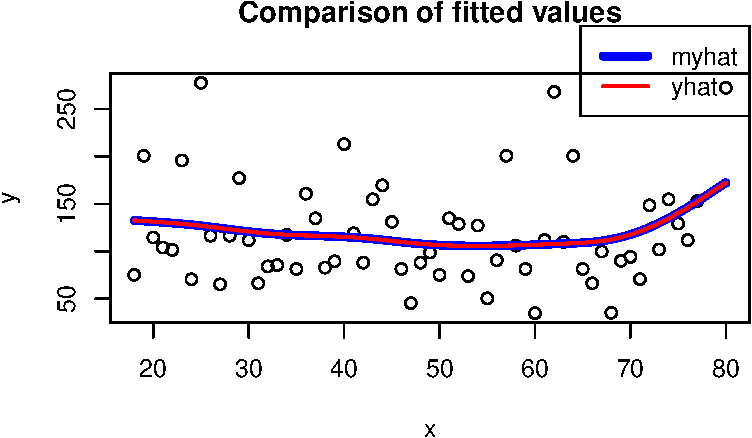
\includegraphics{4Classif_files/figure-beamer/unnamed-chunk-8-1.pdf}

\end{frame}

\begin{frame}

\begin{block}{How to choose \(K\)?}

\vspace{2mm}

\begin{itemize}
\item
  For \(K=1\) the classification is made to the same class as the one
  nearest neighbor. As \(K\) gets very large, the decision boundary
  tends towards a straight line (which is the Bayes boundary in this
  set-up).
\item
  Finding the \emph{optimal value} of \(K\): try different values of
  \(K\) and then test the predictive power of the different classifiers,
  for example by cross-validation (Module 5).
\end{itemize}

\begin{center}\includegraphics[width=0.6\linewidth]{4Classif_files/figure-beamer/knnerror1-1} \end{center}

\end{block}

\end{frame}

\begin{frame}

\begin{block}{Bias-variance trade-off in a classification setting}

\vspace{2mm}

Remember the bias-variance trade-off that we discussed in Module 2.
\vspace{2mm}

Considerations: \vspace{2mm}

\begin{itemize}
\item
  A too low value of \(K\) will give a very flexible classifier which
  will fit the training set too well: High variance, low bias, and thus
  poor predictions for new observations due to overfit.
\item
  Choosing a high value for \(K\) makes the classifier loose its
  flexibility: Low variance, high bias.
\end{itemize}

\vspace{2mm}

\(\rightarrow\) Critical to the success of the classifier to choose the
correct level of flexibility (\(K\)).

\end{block}

\end{frame}

\begin{frame}

\begin{block}{The curse of dimensionality}

\vspace{2mm}

\begin{itemize}
\tightlist
\item
  The nearest neighbor classifier can be quite good if the number of
  predictors \(p\) is small and the number of observations \(n\) is
  large. We need enough close neighbors to make a good classification.
\end{itemize}

\vspace{1mm}

\begin{itemize}
\tightlist
\item
  The effectiveness of the KNN classifier falls quickly when the
  dimension of the preditor space is high.
\end{itemize}

\vspace{1mm}

\begin{itemize}
\tightlist
\item
  Why? Because the nearest neighbors tend to be far away in high
  dimensions and the method is no longer local. This is referred to as
  the \emph{curse of dimensionality}.
\end{itemize}

\end{block}

\end{frame}

\begin{frame}{Bayes decision rule - two paradigms}
\protect\hypertarget{bayes-decision-rule---two-paradigms}{}

\vspace{1mm}

Two approaches to estimate \(\text{Pr}(Y=k \mid X=x)\): \vspace{1mm}

\begin{block}{Diagnostic paradigm}

This is what we did so far: The focus was \emph{directly} estimating the
posterior distribution for the classes \[\text{Pr}(Y=k \mid X=x)\ .\]
\textbf{Examples:} Logistic regression. KNN classification.

\vspace{2mm}

\end{block}

\begin{block}{Sampling paradigm}

\begin{itemize}
\tightlist
\item
  Indirect approach: Model the conditional distribution of predictors
  \(f_k(x)=\text{Pr}(X=x \mid Y=k)\) for each class, and the prior
  probabilities \(\pi_k=\text{Pr}(Y=k)\).
\item
  Then classify to the class with the maximal product \(\pi_k f_k(x)\).
  In this paradigm, we need to model the pdf for each class.
\item
  Popular: the multivariate normal distribution!
\end{itemize}

\end{block}

\end{frame}

\begin{frame}

Given a continuous \(X\) and categorical \(Y\), and

\begin{itemize}
\tightlist
\item
  the probability \emph{\textcolor{red}{density}} function
  \(f_k(x) = \text{Pr}(X=x \mid Y=k)\) for \(X\) in class \(k\).
\item
  the \emph{\textcolor{red}{prior}} probability for class \(k\)
  \(\pi_k = \text{Pr}(Y=k)\) is the prior probability.
\end{itemize}

How do we get \(\text{Pr}(Y=k | X=x_0)\)? That is, how can we ``flip''
the conditioning around? \vspace{4mm}

\begin{block}{\textbf{Bayes theorem}}

\vspace{-3mm}

\begin{align*}
p_k(X) = \text{Pr}(Y=k \mid X= x) &= 
\frac{\text{Pr}(X=x \cap Y=k)}{f(x)}\\
&= \frac{ f_k(x) \pi_k}{\sum_{l=1}^K  f_l(x) \pi_l}  \ .
\end{align*}

\end{block}

\end{frame}

\begin{frame}{Discriminant Analysis}
\protect\hypertarget{discriminant-analysis}{}

\vspace{2mm}

\begin{itemize}
\item
  Discriminant analysis is relying on the \emph{sampling paradigm}.
\item
  The approach is to model the distribution of \(X\) in each of the
  classes separately, and then use Bayes theorem to flip things around
  and obtain \(\text{Pr}(Y \mid X)\).
\end{itemize}

\begin{block}{Example}

\vspace{2mm}

Suppose we have observations coming from two classes:

\{\textcolor{green}{green}, \textcolor{orange}{orange}\}

\[X_{\text{green}}\sim \mathcal{N}(-2, 1.5^2) \text{ and }
X_{\text{orange}}\sim \mathcal{N}(2, 1.5^2) \]

\begin{itemize}
\tightlist
\item
  Assume probabilities to be equal, \(\pi_1 = \pi_2 = 0.5\).
\end{itemize}

\end{block}

\end{frame}

\begin{frame}

We plot \(\pi_k f_k(x)\) for the two classes:

\begin{center}\includegraphics[width=0.7\linewidth]{4Classif_files/figure-beamer/gauss1-1} \end{center}

The decision boundary is where the point of intersection of the two
lines is, because here \(\pi_1 f_1(x)=\pi_2 f_2(x)\).

\end{frame}

\begin{frame}

For different priors \(\pi_1 = 0.3\) and \(\pi_2 = 0.7\), the decision
boundary shifts to the left:

\begin{center}\includegraphics[width=0.7\linewidth]{4Classif_files/figure-beamer/gauss2-1} \end{center}

\end{frame}

\begin{frame}

\begin{block}{Why discriminant analysis?}

\vspace{2mm}

\begin{itemize}
\item
  Linear discriminant analysis is more stable than logistic regression
  when

  \begin{itemize}
  \tightlist
  \item
    the classes are well-separated. In that case, the parameter
    estimates for the logistic regression model are very unstable.
  \item
    \(n\) is small and the distribution of the predictors \(X\) is
    approximately normal in each of the classes.
  \end{itemize}
\end{itemize}

\vspace{2mm}

\begin{itemize}
\tightlist
\item
  Moreover, linear discriminant analysis is popular when we have more
  than two response classes, because it also provides low-dimensional
  views of the data.
\end{itemize}

\end{block}

\end{frame}

\begin{frame}{Linear discriminant analysis (LDA) when \(p=1\)}
\protect\hypertarget{linear-discriminant-analysis-lda-when-p1}{}

\begin{itemize}
\item
  Class conditional distributions \(f_k(X)\) are assumed normal
  (Gaussian) for \(k=1,\ldots,K\), that is
  \[f_k(x) = \frac{1}{\sqrt{2\pi}\sigma_k} e^{-\frac{1}{2}\big(\frac{x-\mu_k}{\sigma_k}\big)^2} \]
  has parameters \(\mu_k\) (mean) and \(\sigma_k\) (standard deviation).
\item
  With LDA we assume that all of the classes have the \emph{same
  standard deviation} \(\sigma_k = \sigma\).
\item
  In addition we have prior class probabilites \(\pi_k=\text{Pr}(Y=k)\),
  so that \(\sum_{k=1}^K \pi_k=1\).
\end{itemize}

\end{frame}

\begin{frame}

We can insert the expression for each class distribution into Bayes
formula to obtain the posterior probability
\(p_k(x) = \text{Pr}(Y = k | X = x)\)
\[p_k(x) = \frac{f_k({\boldsymbol x}) \pi_k}{f({\boldsymbol x})}=\frac{\pi_k \frac{1}{\sqrt{2\pi}\sigma} e^{-\frac{1}{2}\big(\frac{x-\mu_k}{\sigma}\big)^2}}{\sum_{l=1}^K \pi_l \frac{1}{\sqrt{2\pi}\sigma} e^{-\frac{1}{2}\big(\frac{x-\mu_l}{\sigma}\big)^2}} \ .\]

Our rule is to classify to the class for which \(p_k(x)\) is largest.

\end{frame}

\begin{frame}

Taking logs, and discarding terms that do not depend on \(k\), we see
that this is equivalent to assigning \(x\) to the class with the largest
\emph{discriminant score} \(\delta_k(x)\):

\[\delta_k(x) = x\cdot \frac{\mu_k}{\sigma^2} - \frac{\mu_k^2}{2 \sigma^2}+\log(\pi_k).\]

\begin{itemize}
\item
  This decision boundaries between the classes are \emph{linear} in
  \(x\).
\item
  For \(K=2\) classes and \(\pi_1=\pi_2\), the decision boundary is at
\end{itemize}

\[x = \frac{\mu_1+ \mu_2}{2} \ .\]

(Show this by setting \(\delta_1(x)=\delta_2(x)\) and resolving for
\(x\).)

\end{frame}

\begin{frame}[fragile]

\begin{block}{Back to our example}

\[X_{\text{green}}\sim \mathcal{N}(-2, 1.5^2) \text{ and }
X_{\text{orange}}\sim \mathcal{N}(2, 1.5^2) \]

\begin{center}\includegraphics[width=0.6\linewidth]{4Classif_files/figure-beamer/gauss4-1} \end{center}

\begin{itemize}
\item
  The Bayes decision boundary is at \(x=0\).
\item
  Bayes error rate: \texttt{round(pnorm(0,2,1.5))}=0.09.
\item
  The Bayes classifier has the lowest test error rate.
\end{itemize}

\end{block}

\end{frame}

\begin{frame}

\vspace{2mm}

In the above example we knew the true distributions \(p_k(X)\) and the
priors \(\pi_k\). But typically we don't know these parameters, we only
have the training data.

Idea: we simply estimate the parameters and plug them into the rule.

\end{frame}

\begin{frame}

\begin{block}{Parameter estimators}

\vspace{2mm}

\begin{itemize}
\item
  Prior probability for class \(k\) is (often) estimated by taking the
  fraction of observations \(n_k\) (out of \(n\)) coming from class
  \(k\): \(\hat{\pi}_k = \frac{n_k}{n}.\)
\item
  The mean value for class \(k\) is simply the sample mean of all
  observations from class \(k\):
  \[\hat{\mu}_k = \frac{1}{n_k}\sum_{i:y_i=k} x_i.\]
\item
  The standard deviation: sample standard deviation across all classes:
  \[\hat{\sigma}^2=\frac{1}{n-K}\sum_{k=1}^K \sum_{i: y_i=k} (x_i-\hat{\mu}_k)^2 = \sum_{k=1}^K \frac{n_k - 1}{n - K} \cdot \hat{\sigma}_k^2.\]
  \(\hat{\sigma}_k\): estimated standard deviation of all observations
  from class \(k\).
\end{itemize}

\textbf{How can we then estimate the goodness of our estimator?}

\end{block}

\end{frame}

\begin{frame}[fragile]

\begin{enumerate}
\tightlist
\item
  Use the training set to estimate parameters and class boundary:
\item
  Use the test set to estimate misclassification rate.
\end{enumerate}

Simulate data and use training data to estimate \(\mu_k\) and
\(\hat\sigma^2\):

\footnotesize

\begin{Shaded}
\begin{Highlighting}[]
\NormalTok{n =}\StringTok{ }\DecValTok{1000}
\NormalTok{pi1 =}\StringTok{ }\NormalTok{pi2 =}\StringTok{ }\FloatTok{0.5}
\NormalTok{mu1 =}\StringTok{ }\DecValTok{-2}
\NormalTok{mu2 =}\StringTok{ }\DecValTok{2}
\NormalTok{sigma =}\StringTok{ }\FloatTok{1.5}
\KeywordTok{set.seed}\NormalTok{(}\DecValTok{1}\NormalTok{)}
\NormalTok{n1train =}\StringTok{ }\KeywordTok{rbinom}\NormalTok{(}\DecValTok{1}\NormalTok{, n, pi1)}
\NormalTok{n2train =}\StringTok{ }\NormalTok{n }\OperatorTok{-}\StringTok{ }\NormalTok{n1train}
\NormalTok{n1test =}\StringTok{ }\KeywordTok{rbinom}\NormalTok{(}\DecValTok{1}\NormalTok{, n, pi1)}
\NormalTok{n2test =}\StringTok{ }\NormalTok{n }\OperatorTok{-}\StringTok{ }\NormalTok{n1test}
\NormalTok{train1 =}\StringTok{ }\KeywordTok{rnorm}\NormalTok{(n1train, mu1, sigma)}
\NormalTok{train2 =}\StringTok{ }\KeywordTok{rnorm}\NormalTok{(n2train, mu2, sigma)}
\NormalTok{test1 =}\StringTok{ }\KeywordTok{rnorm}\NormalTok{(n1test, mu1, sigma)}
\NormalTok{test2 =}\StringTok{ }\KeywordTok{rnorm}\NormalTok{(n2test, mu2, sigma)}
\NormalTok{var2}\FloatTok{.1}\NormalTok{ =}\StringTok{ }\KeywordTok{var}\NormalTok{(train1)}
\NormalTok{var2}\FloatTok{.2}\NormalTok{ =}\StringTok{ }\KeywordTok{var}\NormalTok{(train2)}
\NormalTok{var.pool =}\StringTok{ }\NormalTok{((n1train }\OperatorTok{-}\StringTok{ }\DecValTok{1}\NormalTok{) }\OperatorTok{*}\StringTok{ }\NormalTok{var2}\FloatTok{.1} \OperatorTok{+}\StringTok{ }\NormalTok{(n2train }\OperatorTok{-}\StringTok{ }\DecValTok{1}\NormalTok{) }\OperatorTok{*}\StringTok{ }\NormalTok{var2}\FloatTok{.2}\NormalTok{)}\OperatorTok{/}\NormalTok{(n }\OperatorTok{-}\StringTok{ }\DecValTok{2}\NormalTok{)}
\end{Highlighting}
\end{Shaded}

\end{frame}

\begin{frame}[fragile]

Then set

\[\hat\delta_1(x) = \hat\delta_2(x)\]

and resolve for \(x\) to obtain a decision rule (boundary).

\vspace{2mm}

\textbf{Exercise}: Verify that the following code will give you the
training and test error rates:

\scriptsize

\begin{Shaded}
\begin{Highlighting}[]
\NormalTok{rule =}\StringTok{ }\FloatTok{0.5} \OperatorTok{*}\StringTok{ }\NormalTok{(}\KeywordTok{mean}\NormalTok{(train1) }\OperatorTok{+}\StringTok{ }\KeywordTok{mean}\NormalTok{(train2)) }\OperatorTok{+}\StringTok{ }\NormalTok{var.pool }\OperatorTok{*}\StringTok{ }\NormalTok{(}\KeywordTok{log}\NormalTok{(n2train}\OperatorTok{/}\NormalTok{n) }\OperatorTok{-}\StringTok{ }
\StringTok{    }\KeywordTok{log}\NormalTok{(n1train}\OperatorTok{/}\NormalTok{n))}\OperatorTok{/}\NormalTok{(}\KeywordTok{mean}\NormalTok{(train1) }\OperatorTok{-}\StringTok{ }\KeywordTok{mean}\NormalTok{(train2))}

\KeywordTok{c}\NormalTok{((}\KeywordTok{sum}\NormalTok{(train1 }\OperatorTok{>}\StringTok{ }\NormalTok{rule) }\OperatorTok{+}\StringTok{ }\KeywordTok{sum}\NormalTok{(train2 }\OperatorTok{<}\StringTok{ }\NormalTok{rule))}\OperatorTok{/}\NormalTok{n, (}\KeywordTok{sum}\NormalTok{(test1 }\OperatorTok{>}\StringTok{ }\NormalTok{rule) }\OperatorTok{+}\StringTok{ }\KeywordTok{sum}\NormalTok{(test2 }\OperatorTok{<}\StringTok{ }
\StringTok{    }\NormalTok{rule))}\OperatorTok{/}\NormalTok{n)}
\end{Highlighting}
\end{Shaded}

\begin{verbatim}
## [1] 0.105 0.115
\end{verbatim}

\normalsize

This is a rather good performance, compared to the minimal Bayes error
rate. But keep in mind that the LDA classifier relies on the Normal
assumption, and that \(\sigma_k=\sigma\) for all classes is
assumed\footnote{Both of which we knew were fulfilled here.}.

\end{frame}

\begin{frame}[fragile]

\begin{block}{The confusion matrix}

\vspace{2mm}

\begin{itemize}
\item
  The confusion matrix is a table that can show the performance of a
  classifier, given that the true values are known.
\item
  We can make a confusion matrix from the training or test set
\item
  The sum of the diagonal is the total number of correct
  classifications. The sum of all elements off the diagonal is the total
  number of misclassifications.
\end{itemize}

\begin{center}

\begin{tabular}{l|l|l|l|l}
\hline
 & Predicted 1 & Predicted 2 & ... & Predicted K\\
\hline
True 1 & correct & wrong & ... & wrong\\
\hline
True 2 & wrong & correct & ... & wrong\\
\hline
... & ... & ... & ... & ...\\
\hline
True K & wrong & wrong & ... & correct\\
\hline
\end{tabular}
\end{center}

\begin{itemize}
\tightlist
\item
  The confusion matrix can be obtained in \texttt{R} by using the
  \texttt{table} function, or directly using the \texttt{caret} package.
\end{itemize}

\end{block}

\end{frame}

\begin{frame}{Multivariate LDA (\(p>1\))}
\protect\hypertarget{multivariate-lda-p1}{}

\vspace{2mm}

\begin{itemize}
\item
  LDA can be generalized to situations when \(p>1\) covariates are used.
  The decision boundaries are still linear.
\item
  The multivariate normal distribution function:
  \[f(x) = \frac{1}{(2 \pi)^{p/2}|\boldsymbol{\Sigma}|^{1/2}}\exp({-\frac{1}{2}({\boldsymbol x}-\boldsymbol\mu)^T \boldsymbol{\Sigma}^{-1}({\boldsymbol x}-\boldsymbol\mu)})\]
\end{itemize}

\centering

\includegraphics[width=0.7\textwidth,height=\textheight]{../../ISLR/Figures/Chapter4/4.5.png}

\end{frame}

\begin{frame}

\begin{itemize}
\item
  This gives the following expression for the discriminant function:
  \[\delta_k(x) = {\boldsymbol x}^T \boldsymbol{\Sigma}^{-1}\boldsymbol\mu_k - \frac{1}{2}\boldsymbol\mu_k^T \boldsymbol{\Sigma}^{-1}\boldsymbol\mu_k + \log \pi_k.\]
\item
  Note: \(\delta_k(x) = c_{k0} + c_{k1}x_1 + \ldots + c_{kp}x_p\) is a
  linear function in \((x_1,\ldots ,x_p)\).
\end{itemize}

\end{frame}

\begin{frame}

In the compulsory 1 exercise you are going to show that the condition

\[P(Y=0 \,|\, \boldsymbol{X}=\boldsymbol{x}) = P(Y=1  \,|\, \boldsymbol{X}=\boldsymbol{x}) \]

can be expressed as

\[\delta_0({\boldsymbol x}) = \delta_1({\boldsymbol x}) \ .\]

\end{frame}

\begin{frame}

\begin{block}{Back to our synthetic example}

\begin{itemize}
\item
  Consider again our simulation from a bivariate normal distribution
  with mean vectors \(\mu_A = (1, 1)^T\), \(\mu_B = (3, 3)^T\), and
  covariance matrix
  \(\Sigma_A = \Sigma_B = \begin{pmatrix} 2\hspace{2mm} 0 \\ 0 \hspace{2mm} 2 \end{pmatrix}\).
\item
  Aim: Use LDA to classify a new observation \(x_0\) to class \(A\) or
  \(B\).
\end{itemize}

\begin{center}\includegraphics[width=0.6\linewidth]{4Classif_files/figure-beamer/synthAB2-1} \end{center}

\end{block}

\end{frame}

\begin{frame}

\begin{itemize}
\item
  Since \emph{the truth is known here}, we can calculate the Bayes
  boundary and the Bayes error.
\item
  Since we have bivariate normal class distributions with common
  covariance matrix, the optimal boundary is given by LDA, with boundary
  given at \(\delta_A({\boldsymbol x})=\delta_B({\boldsymbol x})\).
\end{itemize}

\[{\boldsymbol x}^T \boldsymbol{\Sigma}^{-1}\boldsymbol\mu_A - \frac{1}{2}\boldsymbol\mu_A^T \boldsymbol{\Sigma}^{-1}\boldsymbol\mu_A + \log \pi_A={\boldsymbol x}^T \boldsymbol{\Sigma}^{-1}\boldsymbol\mu_B - \frac{1}{2}\boldsymbol\mu_B^T \boldsymbol{\Sigma}^{-1}\boldsymbol\mu_B + \log \pi_B\]

\[{\boldsymbol x}^T\boldsymbol{\Sigma}^{-1}(\boldsymbol\mu_A -\boldsymbol\mu_B)-\frac{1}{2}\boldsymbol\mu_A^T \boldsymbol{\Sigma}^{-1}\boldsymbol\mu_A +\frac{1}{2}\boldsymbol\mu_B^T \boldsymbol{\Sigma}^{-1}\boldsymbol\mu_B +\log \pi_A-\log \pi_B=0\]

Inserting numerical values gives \(-x_1-x_2+4=0\), thus a boundary with
functional form \[x_2=4-x_1 \ .\]

\end{frame}

\begin{frame}[fragile]

\begin{block}{Confusion matrix for the synthetic example}

\vspace{2mm}

We can use the Bayes boundary to find the error rate:

\scriptsize

\begin{Shaded}
\begin{Highlighting}[]
\NormalTok{r.pred <-}\StringTok{ }\KeywordTok{ifelse}\NormalTok{(df}\OperatorTok{$}\NormalTok{X2 }\OperatorTok{<}\StringTok{ }\DecValTok{4} \OperatorTok{-}\StringTok{ }\NormalTok{df}\OperatorTok{$}\NormalTok{X1, }\StringTok{"A"}\NormalTok{, }\StringTok{"B"}\NormalTok{)}
\KeywordTok{table}\NormalTok{(}\DataTypeTok{real =}\NormalTok{ df}\OperatorTok{$}\NormalTok{class, r.pred)}
\end{Highlighting}
\end{Shaded}

\begin{verbatim}
##     r.pred
## real  A  B
##    A 82 18
##    B 21 79
\end{verbatim}

\vspace{2mm}
\normalsize

\textbf{However}, again, the Bayes boundary is usually not known, and we
must estimate it from the data.

\end{block}

\end{frame}

\begin{frame}

\textbf{Estimators for p\textgreater{}1:}

\begin{itemize}
\item
  Prior probability for class \(k\) (unchanged from \(p=1\)):
  \(\hat{\pi}_k = \frac{n_k}{n}.\)
\item
  The mean value for class \(k\) is simply the sample mean of all
  observations from class \(k\) (but now these are vectors):
  \[\hat{\boldsymbol{\mu}}_k = \frac{1}{n_k}\sum_{i:y_i=k} {\bf X}_i.\]
\item
  The covariance matrices for each class:
  \[\hat{\boldsymbol{\Sigma}}_k=\frac{1}{n_k-1}\sum_{i:y_i=k} ({\bf X}_i-\hat{\boldsymbol{\mu}}_k ) ({\bf X}_i-\hat{\boldsymbol{\mu}}_k)^T\]
\item
  Pooled version:
  \[\hat{\boldsymbol{\Sigma}}= \sum_{k=1}^K \frac{n_k - 1}{n - K} \cdot \hat{\boldsymbol{\Sigma}}_k.\]
\end{itemize}

Optional:
\href{https://www.math.ntnu.no/emner/TMA4268/2018v/notes/ProofMeanS.pdf}{Proof
that the estimator \(\hat{\boldsymbol{\Sigma}}_k\) is unbiased for each
class (from TMA4267)}. Proof for pooled version not provided.

\end{frame}

\begin{frame}[fragile]

\begin{block}{Analysing the synthetic example with \texttt{lda()}}

\vspace{2mm}

To obtain parameters estimates and an estimated decision boundary, we
can use the \texttt{lda()} function in R.

\scriptsize

\begin{Shaded}
\begin{Highlighting}[]
\NormalTok{r.lda <-}\StringTok{ }\KeywordTok{lda}\NormalTok{(class }\OperatorTok{~}\StringTok{ }\NormalTok{X1 }\OperatorTok{+}\StringTok{ }\NormalTok{X2, df)}
\NormalTok{r.pred <-}\StringTok{ }\KeywordTok{predict}\NormalTok{(r.lda, df)}\OperatorTok{$}\NormalTok{class}
\KeywordTok{table}\NormalTok{(}\DataTypeTok{real =}\NormalTok{ df}\OperatorTok{$}\NormalTok{class, }\DataTypeTok{predicted =}\NormalTok{ r.pred)}
\end{Highlighting}
\end{Shaded}

\begin{verbatim}
##     predicted
## real  A  B
##    A 87 13
##    B 18 82
\end{verbatim}

\normalsize

Note: The training error is smaller than for the Bayes boundary. Why?

\end{block}

\end{frame}

\begin{frame}

\begin{block}{Comparison of the Bayes with the estimated boundary}

\vspace{2mm}

Solid line: Bayes boundary

Dashed line: Estimated boundary \(~\)

\begin{center}\includegraphics[width=0.65\linewidth]{4Classif_files/figure-beamer/synthAB3-1} \end{center}

\end{block}

\end{frame}

\begin{frame}

\begin{block}{Posterior probabilites}

\vspace{2mm}

\begin{itemize}
\item
  Sometimes the probability that an observation comes from a class \(k\)
  is more interesting than the actual classification itself.
\item
  These class probabilities can be estimated from the priors and class
  conditional distributions, or from the discriminant functions:
  \begin{align*}\hat{P}(Y=k | X=\boldsymbol{x})&=
  \frac{\hat{\pi}_k \cdot \frac{1}{(2 \pi)^{p/2}|\hat{\boldsymbol{\Sigma}}|^{1/2}} \exp(-\frac{1}{2}
  (\boldsymbol{x}-\hat{\boldsymbol\mu}_k)^T \hat{\boldsymbol{\Sigma}}^{-1}
  (\boldsymbol{x}-\hat{\boldsymbol\mu}_k))}
  {\sum_{l=1}^K \hat{\pi}_l 
  \frac{1}{(2 \pi)^{p/2}|\hat{\boldsymbol{\Sigma}}|^{1/2}}
  \exp(-\frac{1}{2}
  (\boldsymbol{x}-\hat{\boldsymbol\mu}_l)^T 
  \hat{\boldsymbol{\Sigma}}^{-1}
  (\boldsymbol{x}-\hat{\boldsymbol\mu}_l))}\\
  &=
  \frac{e^{\hat{\delta}_k(\boldsymbol{x})}}{\sum_{l=1}^K e^{\hat{\delta}_l(\boldsymbol{x})}}.\end{align*}
\end{itemize}

\end{block}

\end{frame}

\begin{frame}{Quadratic Discriminant Analysis (QDA)}
\protect\hypertarget{quadratic-discriminant-analysis-qda}{}

\begin{itemize}
\item
  In LDA we assumed that \(\boldsymbol{\Sigma}_k = \boldsymbol{\Sigma}\)
  for all classes.
\item
  In QDA we allow different covariance matrices
  \(\boldsymbol{\Sigma}_k\) for each class, while the predictors are
  still multivariate Gaussian
\end{itemize}

\[X \sim N(\boldsymbol{\mu}_k, \boldsymbol{\Sigma}_k) \ .\]

\begin{itemize}
\item
  The discriminant functions are now given by: \vspace{-3mm}
  \begin{align*} \delta_k({\boldsymbol x}) &= -\frac{1}{2}({\boldsymbol x}-\boldsymbol{\mu}_k)^T \boldsymbol{\Sigma}_k^{-1}({\boldsymbol x}-\boldsymbol{\mu}_k)-\frac{1}{2}\log |\boldsymbol{\Sigma}_k| + \log \pi_k \\ 
  &= -\frac{1}{2} {\boldsymbol x}^T \boldsymbol{\Sigma}_k^{-1}{\boldsymbol x} + {\boldsymbol x}^T \boldsymbol{\Sigma}_k^{-1}\boldsymbol{\mu}_k - \frac{1}{2} \boldsymbol{\mu}_k^T \boldsymbol{\Sigma}_k^{-1}\boldsymbol{\mu}_k - \frac{1}{2}\log |\boldsymbol{\Sigma}_k | + \log \pi_k.\\
  \end{align*}
\item
  These decision boundaries are \emph{quadratic} functions of
  \({\boldsymbol x}\).
\end{itemize}

\end{frame}

\begin{frame}

\begin{block}{LDA vs QDA}

\vspace{2mm}

QDA is more flexible than LDA, as it allows for group-specific
covariance matrices.

\vspace{4mm}

\textbf{Q:}

\begin{itemize}
\tightlist
\item
  But, if the covariance matrices in theory are equal - will they not be
  estimated equal?
\item
  Should we not always prefer QDA to LDA?
\end{itemize}

\end{block}

\end{frame}

\begin{frame}

\textbf{A:}

Explanation similar to a ``Bias-variance trade-off'':

\begin{itemize}
\tightlist
\item
  If the assumption of equal covariance matrices is wrong, then LDA may
  suffer from high bias for the parameter estimators.
\item
  But for small sample sizes the covariance matrices might be poorly
  estimated (high variance of estimators).
\end{itemize}

If the number of covariates is high:

\begin{itemize}
\tightlist
\item
  then QDA requires estimating \(K\cdot p \cdot (p+1)/2\) parameters,
\item
  while LDA only requires \(p\cdot(p+1)/2\).
\end{itemize}

Therefore, LDA is less flexible than QDA and might therefore have much
less variance.

\end{frame}

\begin{frame}

\begin{block}{LDA vs QDA -- Illustration}

\vspace{1mm}

Bayes (purple dashed), LDA (black dotted) and QDA (green solid) decision
boundaries for the cases where
\(\boldsymbol{\Sigma}_1 = \boldsymbol{\Sigma}_2\) (left) and
\(\boldsymbol{\Sigma}_1 \neq \boldsymbol{\Sigma}_2\) (right).

\centering

\includegraphics[width=1\textwidth,height=\textheight]{../../ISLR/Figures/Chapter4/4.9.png}

\end{block}

\end{frame}

\begin{frame}[fragile]

\begin{block}{Example: Which type of iris species?}

\vspace{2mm}

The \texttt{iris} flower data set was introduced by the British
statistician and biologist Ronald Fisher in 1936.

\begin{itemize}
\tightlist
\item
  \textbf{Three plant species}: \{setosa, virginica, versicolor\}.
\item
  \textbf{Four features}: \texttt{Sepal.Length}, \texttt{Sepal.Width},
  \texttt{Petal.Length} and \texttt{Petal.Width}.
\end{itemize}

\begin{figure}
\includegraphics[width=0.3\linewidth]{iris} \caption{Iris plant with sepal and petal leaves}\label{fig:iris_pic}
\end{figure}
\vspace{-2mm}
\tiny

\url{http://blog.kaggle.com/2015/04/22/scikit-learn-video-3-machine-learning-first-steps-with-the-iris-dataset/}

\end{block}

\end{frame}

\begin{frame}[fragile]

\begin{block}{Example: Classification of iris plants}

\vspace{2mm}

We will use \texttt{sepal\ width} and \texttt{sepal\ length} to build a
classificator. We have 50 observations from each class.

\scriptsize

\begin{Shaded}
\begin{Highlighting}[]
\KeywordTok{attach}\NormalTok{(iris)}
\KeywordTok{head}\NormalTok{(iris)}
\end{Highlighting}
\end{Shaded}

\begin{verbatim}
##   Sepal.Length Sepal.Width Petal.Length Petal.Width Species
## 1          5.1         3.5          1.4         0.2  setosa
## 2          4.9         3.0          1.4         0.2  setosa
## 3          4.7         3.2          1.3         0.2  setosa
## 4          4.6         3.1          1.5         0.2  setosa
## 5          5.0         3.6          1.4         0.2  setosa
## 6          5.4         3.9          1.7         0.4  setosa
\end{verbatim}

\end{block}

\end{frame}

\begin{frame}

\begin{center}\includegraphics[width=1\linewidth]{4Classif_files/figure-beamer/iris1-1} \end{center}

\end{frame}

\begin{frame}[fragile]

\begin{block}{Iris: LDA}

\scriptsize

\begin{Shaded}
\begin{Highlighting}[]
\NormalTok{iris_lda =}\StringTok{ }\KeywordTok{lda}\NormalTok{(Species }\OperatorTok{~}\StringTok{ }\NormalTok{Sepal.Length }\OperatorTok{+}\StringTok{ }\NormalTok{Sepal.Width, }\DataTypeTok{data =}\NormalTok{ iris, }\DataTypeTok{prior =} \KeywordTok{c}\NormalTok{(}\DecValTok{1}\NormalTok{, }
    \DecValTok{1}\NormalTok{, }\DecValTok{1}\NormalTok{)}\OperatorTok{/}\DecValTok{3}\NormalTok{)}
\end{Highlighting}
\end{Shaded}

\begin{center}\includegraphics[width=0.8\linewidth]{4Classif_files/figure-beamer/iris2-1} \end{center}

\end{block}

\end{frame}

\begin{frame}[fragile]

\begin{block}{Iris: QDA}

\scriptsize

\begin{Shaded}
\begin{Highlighting}[]
\NormalTok{iris_qda =}\StringTok{ }\KeywordTok{qda}\NormalTok{(Species }\OperatorTok{~}\StringTok{ }\NormalTok{Sepal.Length }\OperatorTok{+}\StringTok{ }\NormalTok{Sepal.Width, }\DataTypeTok{data =}\NormalTok{ iris, }\DataTypeTok{prior =} \KeywordTok{c}\NormalTok{(}\DecValTok{1}\NormalTok{, }
    \DecValTok{1}\NormalTok{, }\DecValTok{1}\NormalTok{)}\OperatorTok{/}\DecValTok{3}\NormalTok{)}
\end{Highlighting}
\end{Shaded}

\begin{center}\includegraphics[width=0.8\linewidth]{4Classif_files/figure-beamer/iris3-1} \end{center}

\end{block}

\end{frame}

\begin{frame}[fragile]

\begin{block}{Iris: compare LDA and QDA}

\vspace{2mm}

To compare the \emph{predictive performance} of our two classifiers we
divide the original \texttt{iris} data set randomly into train and test
samples of equal size:

\scriptsize

\begin{Shaded}
\begin{Highlighting}[]
\KeywordTok{set.seed}\NormalTok{(}\DecValTok{1}\NormalTok{)}
\NormalTok{train =}\StringTok{ }\KeywordTok{sample}\NormalTok{(}\DecValTok{1}\OperatorTok{:}\DecValTok{150}\NormalTok{, }\DecValTok{75}\NormalTok{)}

\NormalTok{iris_train =}\StringTok{ }\NormalTok{iris[train, ]}
\NormalTok{iris_test =}\StringTok{ }\NormalTok{iris[}\OperatorTok{-}\NormalTok{train, ]}
\end{Highlighting}
\end{Shaded}

\normalsize

Run LDA and QDA \emph{on the same training set}:

\scriptsize

\begin{Shaded}
\begin{Highlighting}[]
\NormalTok{iris_lda2 =}\StringTok{ }\KeywordTok{lda}\NormalTok{(Species }\OperatorTok{~}\StringTok{ }\NormalTok{Sepal.Length }\OperatorTok{+}\StringTok{ }\NormalTok{Sepal.Width, }\DataTypeTok{data =}\NormalTok{ iris_train, }
    \DataTypeTok{prior =} \KeywordTok{c}\NormalTok{(}\DecValTok{1}\NormalTok{, }\DecValTok{1}\NormalTok{, }\DecValTok{1}\NormalTok{)}\OperatorTok{/}\DecValTok{3}\NormalTok{)}

\NormalTok{iris_qda2 =}\StringTok{ }\KeywordTok{qda}\NormalTok{(Species }\OperatorTok{~}\StringTok{ }\NormalTok{Sepal.Length }\OperatorTok{+}\StringTok{ }\NormalTok{Sepal.Width, }\DataTypeTok{data =}\NormalTok{ iris_train, }
    \DataTypeTok{prior =} \KeywordTok{c}\NormalTok{(}\DecValTok{1}\NormalTok{, }\DecValTok{1}\NormalTok{, }\DecValTok{1}\NormalTok{)}\OperatorTok{/}\DecValTok{3}\NormalTok{)}
\end{Highlighting}
\end{Shaded}

\end{block}

\end{frame}

\begin{frame}[fragile]

LDA training error: \(\frac{14}{75} =0.19\)

\scriptsize

\begin{Shaded}
\begin{Highlighting}[]
\KeywordTok{table}\NormalTok{(}\KeywordTok{predict}\NormalTok{(iris_lda2, }\DataTypeTok{newdata =}\NormalTok{ iris_train)}\OperatorTok{$}\NormalTok{class, iris_train}\OperatorTok{$}\NormalTok{Species)}
\end{Highlighting}
\end{Shaded}

\begin{verbatim}
##             
##              setosa versicolor virginica
##   setosa         27          0         0
##   versicolor      1         15         8
##   virginica       0          5        19
\end{verbatim}

\normalsize

\vspace{2mm}

LDA test error: \(\frac{19}{75} =0.26.\)

\scriptsize

\begin{Shaded}
\begin{Highlighting}[]
\NormalTok{iris_lda2_predict =}\StringTok{ }\KeywordTok{predict}\NormalTok{(iris_lda2, }\DataTypeTok{newdata =}\NormalTok{ iris_test)}
\KeywordTok{table}\NormalTok{(iris_lda2_predict}\OperatorTok{$}\NormalTok{class, iris}\OperatorTok{$}\NormalTok{Species[}\OperatorTok{-}\NormalTok{train])}
\end{Highlighting}
\end{Shaded}

\begin{verbatim}
##             
##              setosa versicolor virginica
##   setosa         22          0         0
##   versicolor      0         22        11
##   virginica       0          8        12
\end{verbatim}

\end{frame}

\begin{frame}[fragile]

QDA training error: \(\frac{13}{75} =0.17\).

\scriptsize

\begin{Shaded}
\begin{Highlighting}[]
\KeywordTok{table}\NormalTok{(}\KeywordTok{predict}\NormalTok{(iris_qda2, }\DataTypeTok{newdata =}\NormalTok{ iris_train)}\OperatorTok{$}\NormalTok{class, iris_train}\OperatorTok{$}\NormalTok{Species)}
\end{Highlighting}
\end{Shaded}

\begin{verbatim}
##             
##              setosa versicolor virginica
##   setosa         28          0         0
##   versicolor      0         16         9
##   virginica       0          4        18
\end{verbatim}

\normalsize

\vspace{2mm}

QDA test error: \(\frac{24}{75}=0.32\).

\scriptsize

\begin{Shaded}
\begin{Highlighting}[]
\NormalTok{iris_qda2_predict =}\StringTok{ }\KeywordTok{predict}\NormalTok{(iris_qda2, }\DataTypeTok{newdata =}\NormalTok{ iris_test)}
\KeywordTok{table}\NormalTok{(iris_qda2_predict}\OperatorTok{$}\NormalTok{class, iris}\OperatorTok{$}\NormalTok{Species[}\OperatorTok{-}\NormalTok{train])}
\end{Highlighting}
\end{Shaded}

\begin{verbatim}
##             
##              setosa versicolor virginica
##   setosa         22          0         0
##   versicolor      0         18        12
##   virginica       0         12        11
\end{verbatim}

\end{frame}

\begin{frame}

\textbf{Result}: The LDA classifier has given the smallest test
error\footnote{Note that the training error is of much less interest; it could be low due to \emph{overfitting} only.}
for classifying iris plants based on sepal width and sepal length for
our test set and should be preferred in this case.

\vspace{2mm}

But:

\begin{enumerate}
\tightlist
\item
  Would another division of the data into training and test set give the
  same conclusion (that LDA is better than QDA for this data set)? (A:
  Not necessarily, but probably.)

  \begin{itemize}
  \tightlist
  \item
    We will look into other choice than dividing into one training and
    one test set in Module 5 (cross-validation).
  \end{itemize}
\end{enumerate}

\vspace{2mm}

\begin{enumerate}
\setcounter{enumi}{1}
\tightlist
\item
  What about the other two covariates? Would adding them to the model (4
  covariates) give a better classification rule? (A: Probably. Try if
  you want.)
\end{enumerate}

\end{frame}

\begin{frame}

\begin{block}{Different forms of discriminant analysis}

\begin{itemize}
\item
  LDA
\item
  QDA
\item
  Naive Bayes (``Idiot's Bayes''): Assume that each class density is the
  product of marginal densities - i.e.~inputs are conditionally
  independent in each class \[f_k(x)=\prod_{j=1}^p f_{kj}(x_j) \ .\]
  This is generally not true, but it simplifies the estimation
  dramatically.
\item
  Other forms by proposing specific density models for \(f_k(x)\),
  including nonparametric approaches.
\end{itemize}

\end{block}

\end{frame}

\begin{frame}

\begin{block}{Naive Bayes}

\begin{itemize}
\item
  Naive Bayes is method that is popular when \(p\) is large.
\item
  The \emph{original naive Bayes}: univariate normal marginal
  distributions. Consequently
  \[\delta_k (x) \propto \log \left[ \pi_i \prod_{j=1}^p f_{kj}(x_j) \right] = - \frac{1}{2} \sum_{j=1}^p \frac{(x_j - \mu_{kj})^2}{\sigma_{kj}^2} + \log(\pi_k) \ , \]
  thus \(\boldsymbol{\Sigma}_k\) is assumed diagonal, and only the
  diagonal elements are estimated.
\item
  Arbitraty generalizations can be made. For example, mixed features
  (qualitative and quantitative predictors).
\item
  This method often produces good results, even though the joint pdf is
  not the product of the marginal pdf. This might be because we are not
  focussing on estimation of class pdfs, but class boundaries.
\end{itemize}

\end{block}

\end{frame}

\begin{frame}

\begin{block}{Summary of Classification Methods}

\begin{itemize}
\item
  Logistic regression
\item
  KNN
\item
  Linear discriminant analysis
\item
  Quadratic discriminant analysis
\item
  Naive Bayes
\end{itemize}

\vspace{4mm}

Remember:

\begin{itemize}
\tightlist
\item
  Logistic regression and KNN \emph{\textcolor{red}{directly estimate}}
  \(\text{Pr}(Y=k \mid X=x)\) (diagnostic paradigm).
\item
  LDA, QDA and naive Bayes \emph{\textcolor{red}{indirectly estimate}}
  \(\text{Pr}(Y=k \mid X=x) \propto f_k(x) \cdot \pi_k\) (sampling
  paradigm).
\end{itemize}

\vspace{2mm}

\end{block}

\end{frame}

\begin{frame}{Which classification method is the best?}
\protect\hypertarget{which-classification-method-is-the-best}{}

\begin{block}{Advantages of discriminant analysis}

\begin{itemize}
\tightlist
\item
  Discriminant analysis is more stable than logistic regression when the
  classes are well-separated.
\item
  Discriminant analysis is more stable than logistic regression if the
  number of observations \(n\) is small and the distribution of the
  predictors \(X\) is approximately (multivariate) normal.
\end{itemize}

\end{block}

\end{frame}

\begin{frame}

\begin{block}{Linearity}

\vspace{2mm}

Assume a binary classification problem with one covariate.

\begin{itemize}
\item
  Recall that logistic regression can be written:
  \[\log \Big ( \frac{p(x)}{1-p(x)}\Big ) = \beta_0 + \beta_1 x.\]
\item
  For a two-class problem, one can show that for LDA
  \[\log\left(\frac{p_1(x)}{1-p_1(x)}\right) = \log\left(\frac{p_1(x)}{p_2(x)}\right) = c_0 + c_1 x_1 \ ,\]
  thus the same linear form. The difference is in how the parameters are
  estimated.
\end{itemize}

\end{block}

\end{frame}

\begin{frame}

\begin{block}{LDA vs logistic regression}

\begin{itemize}
\item
  Logistic regression uses the conditional likelihood based on
  \(\text{Pr}(Y \mid X)\).
\item
  LDA uses the full likelihood based on \(\text{Pr}(X,Y)\).
\item
  Despite these differences, in practice the results are often very
  similar\footnote{logistic regression can also fit quadratic boundaries
  like QDA, by explicitly including quadratic terms in the model.}, but

  \begin{itemize}
  \tightlist
  \item
    LDA is ``more available'' in the multi-class setting.
  \item
    if the class conditional distributions are multivariate normal then
    LDA (or QDA) is preferred.
  \item
    logistic regression makes no assumptions about the covariates and is
    therefore to be preferred in many practical applications.
  \item
    in medicine for two-class problems logistic regression is often
    preferred (for interpretability) and (always) together with ROC and
    AUC (for model comparison).
  \end{itemize}
\end{itemize}

\end{block}

\begin{block}{and KNN?}

\begin{itemize}
\tightlist
\item
  KNN is used when the class boundaries are non-linear.
\end{itemize}

\end{block}

\end{frame}

\begin{frame}

\begin{block}{So: Which classification method is the best?}

\vspace{2mm}

The answer is: \textbf{it depends!}

\begin{itemize}
\item
  Logistic regression is very popular for classification, especially
  when \(K = 2\).
\item
  LDA is useful when \(n\) is small, or the classes are well separated,
  and Gaussian assumptions are reasonable. Also when \(K > 2\).
\item
  Naive Bayes is useful when \(p\) is very large.
\item
  KNN is completely different, as it makes no assumptions about the
  decision boundary nor the distribution of the variables
  (nonparametric). It is expected to work better than LDA and logistic
  regression when boundary is very non-linear. Caveat: No interpretation
  of the effect of the covariates possbile.
\end{itemize}

\vspace{2mm}

Please read Section 4.5 of our coursebook (James et al. 2013).

\end{block}

\end{frame}

\begin{frame}{Two-class problems: sensitivity, specificity}
\protect\hypertarget{two-class-problems-sensitivity-specificity}{}

\begin{itemize}
\item
  Problems with only two classes (binary classifiers) have a special
  status, e.g.~in medicine or biology.
\item
  Assume the classes (\(Y\)) are labelled ``-'' (non disease, or
  \(Y=0\)) and ``+'' (disease, or \(Y=1\)), and that a diagnostic test
  is used to predict \(Y\) given \(X=x\).
\item
  \textbf{Sensitivity} is the proportion of correctly classified
  positive observations:
  \[\frac{\# \text{True Positive}}{\# \text{Condition Positive}}=\frac{\text{TP}}{\text{P}} \ .\]
\item
  \textbf{Specificity} is the proportion of correctly classified
  negative observations:
  \[\frac{\# \text{True Negative}}{\# \text{Condition Negative}}=\frac{\text{TN}}{\text{N}} \ .\]
\end{itemize}

\end{frame}

\begin{frame}

\begin{itemize}
\tightlist
\item
  We would like that a classification rule (or a diagnostic test) have
  both a high sensitivity and a high specificity.
\item
  However, in an imperfect test (i.e., an imperfect predictor) one
  usually comes at the cost of the other.
\end{itemize}

\(2 \times 2\) table shows data from a simple diagnostic study:

\begin{center}
\begin{tabular}{ll|c|c|c}
& & \multicolumn{2}{c}{\emph{Predicted}} \\
& & $Y=0$ & $Y=1$ \\ 
\hline
\multirow{2}{*}{\emph{True}} & $Y=0$ & True negative ($TN$) & False positive ($FN$) & $N$\\
 & $Y=1$ & False negative ($FP$) & True positive ($TP$) & $P$\\
\hline
& & $N^\star$ & $P^\star$ & $Tot$ 
\end{tabular}
\end{center}

\end{frame}

\begin{frame}[fragile]

\begin{block}{Example Continued: South African heart disease}

\vspace{2mm}

We evaluate our multiple logistic model for the \texttt{SAheart} data
set. To investigate the training error and the test error, we divide the
original data set randomly into two samples of equal size.

\scriptsize

\begin{Shaded}
\begin{Highlighting}[]
\KeywordTok{set.seed}\NormalTok{(}\DecValTok{20}\NormalTok{)}
\NormalTok{train_ID =}\StringTok{ }\KeywordTok{sample}\NormalTok{(}\DecValTok{1}\OperatorTok{:}\KeywordTok{nrow}\NormalTok{(d.heart), }\KeywordTok{nrow}\NormalTok{(d.heart)}\OperatorTok{/}\DecValTok{2}\NormalTok{)}
\NormalTok{train_SA =}\StringTok{ }\NormalTok{d.heart[train_ID, ]}
\NormalTok{test_SA =}\StringTok{ }\NormalTok{d.heart[}\OperatorTok{-}\NormalTok{train_ID, ]}
\end{Highlighting}
\end{Shaded}

\normalsize

\textbf{Fit} a logistic regression model, \textbf{using the training set
only}:

\scriptsize

\begin{Shaded}
\begin{Highlighting}[]
\NormalTok{glm_SA =}\StringTok{ }\KeywordTok{glm}\NormalTok{(chd }\OperatorTok{~}\StringTok{ }\NormalTok{., }\DataTypeTok{data =}\NormalTok{ train_SA, }\DataTypeTok{family =} \StringTok{"binomial"}\NormalTok{)}
\KeywordTok{summary}\NormalTok{(glm_SA)}\OperatorTok{$}\NormalTok{coef}
\end{Highlighting}
\end{Shaded}

\begin{verbatim}
##                     Estimate  Std. Error     z value    Pr(>|z|)
## (Intercept)    -3.7674748108 1.439119254 -2.61790314 0.008847191
## sbp             0.0045154473 0.008907046  0.50695226 0.612188315
## tobacco         0.1253783872 0.043828325  2.86067029 0.004227464
## ldl             0.0484641791 0.080453775  0.60238540 0.546917627
## famhistPresent  0.8186419234 0.338067955  2.42153068 0.015455296
## obesity        -0.0226110199 0.040483169 -0.55852890 0.576483276
## alcohol        -0.0007383597 0.008039590 -0.09184047 0.926824793
## age             0.0446073935 0.014781896  3.01770439 0.002546972
\end{verbatim}

\end{block}

\end{frame}

\begin{frame}[fragile]

\begin{itemize}
\tightlist
\item
  The estimated probability of a \texttt{chd} event (\(Y=1\)) is then
  given as \[\hat{p}(\mathbf{X}) =\frac{e^\eta}{1+e^\eta} ,\] with
  \(\eta=\beta_0 + \beta_1 \cdot x_{\text{sbp}} + \beta_2\cdot x_{\text{tobacco}} + \beta_3 \cdot x_\text{ldh} + \beta_4 \cdot x_{famhist} + \beta_5\cdot x_\text{obesity} + \beta_6\cdot x_\text{alcohol} + \beta_7\cdot x_{\text{age}}\).
\end{itemize}

\hspace{6mm}

Remember that \(x_{famhist} \in \{0,1\}\) is a binary covariate.

\vspace{2mm}

\begin{itemize}
\tightlist
\item
  We are interested in the \textbf{predictions for the test set}
  (although it is of course possible to calculate predictions for the
  training set, too).
\end{itemize}

\end{frame}

\begin{frame}[fragile]

\begin{itemize}
\tightlist
\item
  The \texttt{predict} function does these calculations for us. When
  specifying \texttt{type="response"} the function returns the
  probabilities for \(Y=1\).
\end{itemize}

\scriptsize

\begin{Shaded}
\begin{Highlighting}[]
\NormalTok{probs_SA =}\StringTok{ }\KeywordTok{predict}\NormalTok{(glm_SA, }\DataTypeTok{newdata =}\NormalTok{ test_SA, }\DataTypeTok{type =} \StringTok{"response"}\NormalTok{)}
\end{Highlighting}
\end{Shaded}

\normalsize

\begin{itemize}
\tightlist
\item
  Classifications are obtained by specifying a threshold value. We have
  here chosen a threshold value of 0.5. By using the \texttt{ifelse}
  function we specify that all probabilities larger than 0.5 are to be
  classified as 1, while the remaining probabilities are to be
  classified as 0.
\end{itemize}

\end{frame}

\begin{frame}[fragile]

\scriptsize

\begin{Shaded}
\begin{Highlighting}[]
\NormalTok{pred_SA =}\StringTok{ }\KeywordTok{ifelse}\NormalTok{(probs_SA }\OperatorTok{>}\StringTok{ }\FloatTok{0.5}\NormalTok{, }\DecValTok{1}\NormalTok{, }\DecValTok{0}\NormalTok{)}

\NormalTok{predictions_SA =}\StringTok{ }\KeywordTok{data.frame}\NormalTok{(probs_SA, pred_SA, test_SA[, }\StringTok{"chd"}\NormalTok{])}
\KeywordTok{colnames}\NormalTok{(predictions_SA) =}\StringTok{ }\KeywordTok{c}\NormalTok{(}\StringTok{"Estim. prob. of Y=1"}\NormalTok{, }\StringTok{"Predicted class"}\NormalTok{, }
    \StringTok{"True class"}\NormalTok{)}
\KeywordTok{head}\NormalTok{(predictions_SA)}
\end{Highlighting}
\end{Shaded}

\begin{verbatim}
##    Estim. prob. of Y=1 Predicted class True class
## 1            0.7741048               1          1
## 4            0.7141807               1          1
## 7            0.2258178               0          0
## 11           0.5216856               1          1
## 12           0.7112496               1          1
## 15           0.6702761               1          0
\end{verbatim}

\end{frame}

\begin{frame}[fragile]

The confusion matrix is used to count the number of misclassifications
in the test set:

\scriptsize

\begin{Shaded}
\begin{Highlighting}[]
\KeywordTok{table}\NormalTok{(}\DataTypeTok{predicted =}\NormalTok{ pred_SA, }\DataTypeTok{true =}\NormalTok{ d.heart[}\OperatorTok{-}\NormalTok{train_ID, }\StringTok{"chd"}\NormalTok{])}
\end{Highlighting}
\end{Shaded}

\begin{verbatim}
##          true
## predicted   0   1
##         0 118  45
##         1  27  41
\end{verbatim}

\normalsize

\begin{itemize}
\tightlist
\item
  The logistic model has correctly classified 118+41 times, and
  misclassified 27+45 times, thus
  \[\text{Test error rate} = \frac{27+45}{27+45+118+41} \approx 0.31 \ .\]
\item
  Sensitivity: \(\frac{41}{41+27}=0.603\), specificity =
  \(\frac{118}{118+45}=0.724.\)
\end{itemize}

\end{frame}

\begin{frame}

\begin{block}{ROC curves and AUC}

\vspace{2mm}

\begin{itemize}
\item
  The receiver operating characteristics (ROC) curve gives a graphical
  display of the sensitivity against (1-specificity), as the threshold
  value (cut-off on probability of success or disease) is moved over the
  range of all possible values.
\item
  An ideal classifier will give a ROC curve which hugs the top left
  corner (sensitivity = specificity = 1), while a straight line
  represents a classifier with a random guess of the outcome.
\item
  The \textbf{AUC} score is the area under the AUC curve. It ranges
  between the values 0 and 1, where a higher value indicates a better
  classifier.
\item
  The AUC score is useful for comparing the performance of different
  classifiers, as all possible threshold values are taken into account.
\end{itemize}

\end{block}

\end{frame}

\begin{frame}

\begin{block}{Example Continued: South African heart disease}

In order to see how our model performs for different threshold values,
we can plot a ROC curve:

\scriptsize

\begin{center}\includegraphics[width=0.8\linewidth]{4Classif_files/figure-beamer/roc-1} \end{center}

\end{block}

\end{frame}

\begin{frame}[fragile]

To check where in the plot we find the default cut-off on 0.5, we need
to calculate sensitivity and specificity for this cut-off:

\scriptsize

\begin{Shaded}
\begin{Highlighting}[]
\NormalTok{res =}\StringTok{ }\KeywordTok{table}\NormalTok{(pred_SA, d.heart[}\OperatorTok{-}\NormalTok{train_ID, }\StringTok{"chd"}\NormalTok{])}
\NormalTok{sens =}\StringTok{ }\NormalTok{res[}\DecValTok{2}\NormalTok{, }\DecValTok{2}\NormalTok{]}\OperatorTok{/}\KeywordTok{sum}\NormalTok{(res[}\DecValTok{2}\NormalTok{, ])}
\NormalTok{spec =}\StringTok{ }\NormalTok{res[}\DecValTok{1}\NormalTok{, }\DecValTok{1}\NormalTok{]}\OperatorTok{/}\KeywordTok{sum}\NormalTok{(res[}\DecValTok{1}\NormalTok{, ])}
\NormalTok{sens}
\end{Highlighting}
\end{Shaded}

\begin{verbatim}
## [1] 0.6029412
\end{verbatim}

\begin{Shaded}
\begin{Highlighting}[]
\NormalTok{spec}
\end{Highlighting}
\end{Shaded}

\begin{verbatim}
## [1] 0.7239264
\end{verbatim}

\normalsize

Observe that the value 0.603 (on \(y\)-axis) and 0.276 (1-specificity on
\(x\)-axis) is on our ROC curve.

The ROC-curve is made up of all possible cut-offs and their associated
sensitivity and specificity.

\end{frame}

\begin{frame}{Further reading}
\protect\hypertarget{further-reading}{}

\begin{itemize}
\tightlist
\item
  \href{https://www.youtube.com/playlist?list=PL5-da3qGB5IC4vaDba5ClatUmFppXLAhE}{Videoes
  on YouTube by the authors of ISL, Chapter 4, plus the videos for KNN
  in Chapter 2}
\end{itemize}

\end{frame}

\begin{frame}

\begin{block}{Want to learn more (theory) about logistic regression?}

\begin{itemize}
\item
  In TMA4315 Generalized linear models there are 3 weeks with binary
  regression - mainly logistic regression:
  \href{https://www.math.ntnu.no/emner/TMA4315/2018h/3BinReg.html}{TMA4315M3:
  Binary regression}.
\item
  The focus there is on all parts of the regression (not classification)
  with a mathematical focus on estimation, inference, model fit.
\end{itemize}

\end{block}

\end{frame}

\begin{frame}{References}
\protect\hypertarget{references}{}

\hypertarget{refs}{}
\leavevmode\hypertarget{ref-james.etal}{}%
James, G., D. Witten, T. Hastie, and R. Tibshirani. 2013. \emph{An
Introduction to Statistical Learning with Applications in R}. New York:
Springer.

\end{frame}

\end{document}
